% ------------------------------------------------

% Basic configuration
% 基本設定
\documentclass[12pt, a4paper]{report}

% ------------------------------------------------

% XeLaTex 的設定

% --------------------------
%加這個就可以設定字體
\usepackage{fontspec}

%使用xeCJK,其他的還有CJK或是xCJK
\usepackage{xeCJK}

% Set english font
\setmainfont{Times New Roman} % In Windows
%\usepackage{times} % In *nix 

%設定中英文的字型
%字型的設定可以使用系統內的字型,而不用像以前一樣另外安裝
\setCJKmainfont{標楷體}

%中文自動換行
\XeTeXlinebreaklocale "zh"

%文字的彈性間距
\XeTeXlinebreakskip = 0pt plus 1pt

%設定段落之間的距離
\setlength{\parskip}{0.3cm}

%設定行距
\linespread{1.5}\selectfont

% ------------------------------------------------

% LaTex package

% --------------------------
\usepackage{graphicx}
%\usepackage{ncku/pdf}
%\usepackage{style/rotating}
\usepackage{./ncku/style/macros}
%\usepackage{style/psfig}
%\usepackage{epsfig}
\usepackage{latexsym}
\usepackage{./ncku/style/utdiss}
\usepackage{hyperref}
%\usepackage{hyperxmp}
\usepackage{pdfpages}

%preamble
%\usepackage[nottoc]{tocbibind}

% ------------------------------------------------

% 有關學校對論文要求的設定

% --------------------------

% 學校浮水印 Watermark
%\usepackage{draftwatermark}
%\SetWatermarkText{}

\AddToShipoutPicture{
\put(0,0){
\parbox[b][\paperheight]{\paperwidth}{
\vfill
\centering
\includegraphics[]{./ncku/watersymbol.jpg}
\vfill
}}}


% --------------------------


% ----------------------------------------------------------------------------
%                           Command for cover page
% ----------------------------------------------------------------------------

% default variables definitions
% 此處只是預設值,不需更改此處
% 請更改 names.tex 內容
\newcommand\cTitle{}
\newcommand\eTitle{}
\newcommand\myCname{}
\newcommand\myEname{}
\newcommand\advisorCnameA{}
\newcommand\advisorEnameA{}
\newcommand\advisorCnameB{}
\newcommand\advisorEnameB{}
\newcommand\advisorCnameC{}
\newcommand\advisorEnameC{}
\newcommand\univCname{}
\newcommand\univEname{}
\newcommand\deptCname{}
\newcommand\fulldeptEname{}
\newcommand\deptEname{}
\newcommand\collEname{}
\newcommand\degreeCname{}
\newcommand\degreeEname{}
\newcommand\cYear{}
\newcommand\cMonth{}
\newcommand\eYear{}
\newcommand\eMonth{}
\newcommand\ePlace{}


% --------------------------

% 論文有關資料
\input{./names.tex}

% --------------------------

% 使用 hyperref 在 pdf 簡介欄裡填入相關資料
\ifx \hypersetup \undefined
	\relax  % do nothing
\else
	\hypersetup
    {
        unicode     = true,
	    pdftitle    = {\eTitle (\cTitle)},
	    pdfauthor   = {\myEname (\myCname)},
        pdfcreator  = {\univEname},
%        pdfproducer = {\univEname},
        pdfsubject  = {},
        pdfkeywords = {},
    }
\fi

% ------------------------------------------------


% ------------------------------------------------

% Start of paper
\begin{document}

% ------------------------------------------------

% 封面 Cover
% 請根據你的需求去選用中文或英文封面
% 活在全球化, 使用英文封面是優先推薦
%%%%%%%%%%%%%%%%%%%%%%%%%%%%%%%
%       NCKU cover 封面
%%%%%%%%%%%%%%%%%%%%%%%%%%%%%%%
%
\begin{titlepage}

% 判斷是否要浮水印?
\ifx\mywatermark\undefined 
  \thispagestyle{empty}  % 無頁碼、無 header (無浮水印)
\else
  \thispagestyle{EmptyWaterMarkPage} % 無頁碼、有浮水印
\fi

% aligned to the center of the page
\begin{center}
% font size (relative to 12 pt):
% \large (14pt) < \Large (18pt) < \LARGE (20pt) < \huge (24pt)< \Huge (24 pt)
%
\makebox[10cm][s]{\Huge\univCname}\\  %顯示中文校名
\vspace{1cm}
\makebox[8cm][s]{\Huge\deptCname}\\ %顯示中文系所名
\vspace{1cm}
\makebox[5cm][s]{\Huge\degreeCname 論文}\\ %顯示論文種類 (中文)
\vspace{1.5cm}
\vspace{2cm}
\vspace{2.5cm}

%
% Set the line spacing to single for the titles (to compress the lines)
\renewcommand{\baselinestretch}{1}   %行距 1 倍
%\large % it needs a font size changing command to be effective
\Large\cTitle\\  % 中文題目
%
\vspace{0.5cm}
%
\Large\eTitle\\ %英文題目

\vspace{3.5cm}

% \makebox is a text box with specified width;
% option s: stretch; option l: left aligned
% use \makebox to make sure
% 「研究生」 與「指導教授」occupy the same width
% Names are filled in a box with pre-defined width
% the left and right sides of 「:」occupy the same width (use \hspace{} to fill the short)
% to guarantee 「:」is at the center
% assume the width of a Chinese character is 1.2em
% 4.8em is determined by the length of the longest string "指導教授"
% 7.2em is determined by the length of the possibly longest name + title "歐陽明志博士"
\hspace{2.4em}%
\makebox[4.8em][s]{\Large 研究生}%
\makebox[1em][c]{\Large :}%
\makebox[7.2em][l]{\Large\myCname}\\  % 顯示作者中文名

\vspace{0.5cm}

\hspace{2.4em}%
\makebox[4.8em][s]{\Large 指導教授}%
\makebox[1em][c]{\Large :}%
\makebox[7.2em][l]{\Large\advisorCnameA}\\  %顯示指導教授A中文名
%
% 判斷是否有共同指導的教授 B
\ifx \advisorCnameB  \itsempty
\relax % 沒有 B 教授,所以不佔版面,不印任何空白
\else
\vspace{0.1cm}
% 共同指導的教授 B
\hspace{2.4em}%
\makebox[4.8em][s]{}%
\makebox[1em][c]{}%
\makebox[7.2em][l]{\Large\advisorCnameB}\\%顯示指導教授B中文名
\fi
%
% 判斷是否有共同指導的教授 C
\ifx \advisorCnameC  \itsempty
\relax % 沒有 C 教授,所以不佔版面,不印任何空白
\else
\vspace{0.1cm}
% 共同指導的教授 C
\hspace{2.4em}%
\makebox[4.8em][s]{}%
\makebox[1em][c]{}%
\makebox[7.2em][l]{\Large\advisorCnameC}\\%顯示指導教授B中文名
\fi
%
\vfill

\vspace{1cm}
\makebox[8cm][s]{\Large 中華民國\cYear 年\cMonth 月}%
%
\end{center}

\end{titlepage}
%%%%%%%%%%%%%%


% ----------------------------------------------------------------------------
%                                English cover
%                                   英文封面
% ----------------------------------------------------------------------------

% Set the line spacing to single for the titles (to compress the lines)
\renewcommand{\baselinestretch}{1}   %行距 1 倍

% ------------------------------------------------

% Page start
\newpage
\phantomsection

% Add to "Table of Contents"
\addcontentsline{toc}{chapter}{Cover}

% 設定使用 無頁碼, 有浮水印
\thispagestyle{empty}

% Aligned to the center of the page
\begin{center}

% ------------------------------------------------

% 顯示 校名, 系所名, 論文種類
\makebox[10cm][c]{\Huge\univEname}\\
\vspace{0.5cm}
\makebox[8cm][c]{\LARGE\fulldeptEname}\\
\vspace{0.5cm}
\makebox[5cm][c]{\LARGE Master's Thesis}\\

% ------------------------------------------------

% Space
\vspace{7cm}

% ------------------------------------------------

% English title 英文題目
\LARGE\eTitle\\
\vspace{4.5cm}

% ------------------------------------------------

% 顯示學生和老師的名字

% --------------------------

% 顯示 學生 的名字
\makebox[4.8em][r]{\Large Student}
\makebox[1em][c]{\Large:}
\makebox[7.2em][l]{\Large\myEname}\\

\vspace{0.5cm}

% --------------------------

% 顯示 老師 (指導老師 A) 的名字
\makebox[4.8em][r]{\Large Advisor}
\makebox[1em][c]{\Large:}
\makebox[7.2em][l]{\Large\advisorEnameA}\\

% --------------------------

% 指導老師 B
\ifx \advisorEnameB  \itsempty
    % 沒有 老師B 的話, 不佔版面和不印任何空白
    \relax
\else
    % 顯示 老師B 的名字
    \vspace{0.1cm}
    \hspace{6.3em}
    \makebox[7.2em][l]{\Large\advisorEnameB}\\
\fi

% --------------------------

% 指導老師 C
\ifx \advisorEnameC  \itsempty
    % 沒有 老師C 的話, 不佔版面和不印任何空白
    \relax
\else
    % 顯示 老師C 的名字
    \vspace{0.1cm}
    \hspace{6.3em}
    \makebox[7.2em][l]{\Large\advisorEnameC}\\
\fi

% ------------------------------------------------

% Date 日期
\vspace{1.1cm}
\makebox[8cm][c]{\Large \eMonth\ \ \eYear}

% ------------------------------------------------

% End of alignment
\end{center}

% End of page

% ------------------------------------------------


% ------------------------------------------------

% 口試証明文件 Document of oral presentation
\begin{figure}[h]
\centering
\vspace{-29mm}
\begin{tabular}{c}
\hspace{-36mm} \includegraphics[]{./oral/oral-chi.pdf}
\end{tabular}
\end{figure}
\newpage
\newpage

\begin{figure}[h]
\centering
\vspace{-29mm}
\begin{tabular}{c}
\hspace{-36mm} \includegraphics[]{./oral/oral-eng.pdf}
\end{tabular}
\end{figure}
\newpage
\newpage


% ------------------------------------------------

% 摘要 Abstract
% 請根據你的需求去選用中文或英文版
%
% 學校要求如果是寫中文版的話
% 則要同時交出英文版
%
% 只交英文版就不用交中文版
%
% 詳細學校的要求可去附件看

% ----------------------------------------------------------------------------
%                               English abstract
%                                   英文摘要
% ----------------------------------------------------------------------------

% Set the line spacing
\baselineskip = 26pt

% ------------------------------------------------

% Page start
\newpage
\phantomsection

% Add to "Table of Contents"
\addcontentsline{toc}{chapter}{Abstract}

% ------------------------------------------------

\begin{center}
\large \textbf{Abstract}
%\label{abstract}
\end{center}

% ------------------------------------------------

%\minisec{Abstract}
%In big data, the meaning of owning one petabyte or ten petabyte are the same --- meaningless. The information is hiding inside the data, this means how fast can the data retrieval from database and process it to become an information we need that is the major question in this field, and normally the bottleneck is the query operation that between the database \cite{paper:nodb} and the program.\\

%To lower the searching time in database, people are start using non-relational database from relational database to seek for less searching time. But this kind of changing may meet some problem, such as re-design the schema of the database. Because non-relational database are using key-value pair design, if you want to retrieve a value, you need to know its key, but you can't using the value to find the key or using conditional searching (like the 'WHERE Clause' in SQL) to search the key or value. This will cause some feature which basic on the query operation un-functional in program, this may need to modify tons of code to become useable. Also if these kind of features are very important and use widely which may need to use MapReduce to distribute the searching into many servers for decreasing the searching times. This is highly increased the work for programmer and system designer, also increased the cost of maintenance the servers.\\

%So this paper is to design a indexing algorithm custom for key-value stores --- Li's Hash, using the original key-value usage to implement a indexing to provide the basic query feature in relational database such as the searching and comparison operation, also the time complexity of these feature is $O(1)$ or $O(b)$ ($b$ is the data's byte length store in Li's Hash).\\

%Because Li's Hash is design as a dynamic indexing algorithm which means the indexing are doing when input a key-value data, rather than normal indexing which needed a freeze state. By using modularized design for swappable the back-end database, we have implemented a prototype to provide as a library \cite{web:lishash:home-page} that let the user can use relational or non-relational APIs with different back-end non-relational database, just only need to modify the code for connecting to our library, then they don't need to modified any schema in original design, and keep the relational database concept to use non-relational database without need to learn any new concept about the back-end database.\\

In age of big data, owning one petabyte or ten petabyte is meaningless, because the storage no longer as primary issue.\\

The information is hiding inside the data, this means how fast can the data retrieval from database and process it to become an information we needed that is the major issue.\\

People are start using non-relational database from relation database to seek for less searching time. But non-relational database are using key-value pair design, if you want to retrieve a value, you need to know its key, but you can't using the value to find the key or using conditional searching (like the 'WHERE Clause' in SQL) to search the key or value. This will cause some feature which basic on the query operation un-functional, also if these kind of features are very important and use widely which may need to use MapReduce to distribute the searching. This will highly increased the work for programmer and cost of maintenance the servers.\\

So this paper is to design a indexing algorithm custom for key-value stores --- Li's Hash, using the original key-value usage to implement a indexing to provide the query feature in relational database such as the searching and comparison operation, also the time complexity of these feature is $O(1)$ or $O(b)$ ($b$ is the data's byte length store in Li's Hash).\\

This paper have implemented a prototype to build up a library in order to provide relational or non-relational APIs with different back-end non-relational database, user only need to modify the code for connecting to this library, then they don't need to modified any schema in original design, and keep the relational database concept to use non-relational database without need to learn any new concept about the back-end database.\\

% ------------------------------------------------

\begin{itemize}
\item {\bf Keywords:} Floorplanning, Bus planning
\end{itemize}

% ------------------------------------------------

% End of page

% ------------------------------------------------


% ----------------------------------------------------------------------------
%                               Chinese abstract
%                                   中文摘要
% ----------------------------------------------------------------------------

% Set the line spacing
%\baselineskip = 26pt

% ------------------------------------------------

% Page start
\newpage
%\cleardoublepage
\phantomsection
\addcontentsline{toc}{chapter}{Abstract}

% ------------------------------------------------

\begin{center}
\large \textbf{摘要}
%\label{abstract}
\end{center}

% ------------------------------------------------

由於在嵌入式系統中,匯流排的數量急劇地上升,匯流排規劃的品質好壞成為決定嵌入式系統效能與系統功率消耗的重要指標。為了不讓匯流排的問題造成晶片設計流程後期的限制,在早期平面佈局時就將匯流排的因素加入考慮是比較理想的處理方式。近年來,匯流排導向平面佈局的問題吸引了許多人的注意,並且已有相當多的方法被提出於處理相關的問題。然而,目前的演算法都採取了比較簡單的問題定義,忽略了匯流排腳位的位置和方向等相關的資訊。忽略了上述的資訊可能會造成系統效能被高估的情況。因此,我們提出了一個匯流排導向的平面佈局演算法,我們所提出的演算法在規劃匯流排時也考慮到腳位的位置與方向的資訊,讓演算法所得到的結果能夠更符合實際情況。由於在規劃匯流排的同時也考慮匯流排腳位的資訊,匯流排轉彎的地方並不局限在匯流排所連接的方塊上。因此,在處理匯流排繞線問題時也比較有彈性。随著整個匯流排拓撲的形狀變得更有彈性,匯流排繞線的成功率也相對地提高,許多較佳的結果就能被發掘出來。將我們的演算法所得到的結果與目前最佳的匯流排導向平面佈局演算法所得到的結果比較,我們演算法的執行時間相對快了3.5倍,繞線成功率提高了1.2倍,匯流排長度少了1.8倍,並且將平面佈局中空白的區域降低了1.2倍。

% ------------------------------------------------

\begin{itemize}
\item {\bf 關鍵字:} 平面規劃, 匯流排規劃
\end{itemize}

% ------------------------------------------------

% End of page

% ------------------------------------------------


% ------------------------------------------------

% 致謝 Acknowledgments
% ------------------------------------------------

\ifthenelse{\GetLangEnableChi = 1}
{
  % ------------------------------------------------
\StartAcknowledgments{chapter:acknowledgments-chi}
% ------------------------------------------------

%感謝那些實驗室和老師的幫助, 可去Acknowledgments{}看詳細說明

"我思故我在, 我做故我存."\\
"I think, therefore I am. I do, therefore I valuable."\\

"別人笑我太瘋癲,我笑他人看不穿."\\
"People laugh at me for my insane, but I laugh them because they don't see the truth."\\

%感謝圖書館的組去查核本模板所產生的樣子適合當成畢業論文, 以讓同學可以安心使用本模板; 另外同時十分感謝一些老師的幫忙和意見, 以讓本模板更完整, 閱讀更清楚.
%那些
%實驗室和老師的幫助, 可去Acknowledgments{}看詳細說明

% ------------------------------------------------
\EndAcknowledgments
% ------------------------------------------------

}{}

\ifthenelse{\GetLangEnableEng = 1}
{
  % ------------------------------------------------
\StartAcknowledgments{chapter:acknowledgments}
% ------------------------------------------------

Thanks someone you want here.

Ask Google\cite{website:google} if you need. (If you set some references file, you need to use at least one cite to make Latex work.)

% ------------------------------------------------
\EndAcknowledgments
% ------------------------------------------------

}{}

% ------------------------------------------------


% ----------------------------------------------------------------------------
%                            Chinese acknowledgments
%                                   中文致謝
% ----------------------------------------------------------------------------

% Set the line spacing
%\baselineskip = 26pt

% ------------------------------------------------

% Page start
\newpage
\phantomsection

% Add to "Table of Contents"
\addcontentsline{toc}{chapter}{Acknowledgments}

% ------------------------------------------------

\begin{center}
\large \textbf{Acknowledgments}
%\label{acknowledgments}
\end{center}

% ------------------------------------------------

"我思故我在, 我做故我存."\\
"I think, therefore I am. I do, that become valuable."\\

"別人笑我太瘋癲,我笑他人看不穿."\\
"People laugh at me for my insane, but I laugh them because they don't see the truth."\\

% ------------------------------------------------

% End of page

% ------------------------------------------------


% ------------------------------------------------

\newpage
\phantomsection
\addcontentsline{toc}{chapter}{Table of Contents}
\tableofcontents

\newpage
\phantomsection
%\addcontentsline{toc}{section}{List of Tables}
\listoftables

\newpage
\phantomsection
%\addcontentsline{toc}{section}{List of Figures} 
\listoffigures

% ------------------------------------------------


%\onehalfspacing

% ------------------------------------------------
\StartChapter{Introduction}{chapter:how-to:write:introduction}
% ------------------------------------------------
\section{基本介紹}

  \begin{framed}
  \begin{verbatim}
    - 參數 -
    空掉: 是指可以寫成{} (即是不寫任何內容), 但是{}必須要存在.
    不填: 是指{}不必存在.

    但如果要使用最後的參數, 中間'可不填'則變成'可空掉',
    否則會錯誤或沒法使用.
  \end{verbatim}
  \end{framed}

這教學包含了原Latex和本模板特有的語法的使用方式和例子.

請注意原Latex語法會以英文小寫來顯示(\verb|\aabbcc|); 而本模板特有的語法會以英文大小寫混合(\verb|\AaBbCc|, 第一個字必定以大寫來顯示), 由於這些特有語法\textbf{不是}原Latex的語法, 所以不能直接應用在非本模板的Latex檔案上.

抄襲就是學習的第一步 (如同我們小時候去抄襲父母走路一樣), 如果你看完本教學都不知道怎樣寫的話, 証明是時候你親自下手實作, 我有留下了一些範本 (在'./context'下)以方便大家開始第一步, 之後就要靠大家自己的努力和實作, 再加上自己的探索能力了.

有問題的話, 可以有以下的地方找尋答案 (請使用這順序):
\begin{enumerate}
\item 直接研究在模板的Latex寫法 (在'./example'以下的所有檔案)
\item 查問懂得Latex的老師和同學 (這種人少得可憐, 可能去問Google老師會更快)
\item 去Wikibook\RefBib{web:latex:wikibooks} (這邊100\%會有你想要的答案, 問題是你會不會懂得使用)
\item 請求Google老師
\end{enumerate}

另外, 如果覺得本教學還缺少了什麼說明, 請告知.

% ------------------------------------------------
\EndChapter
% ------------------------------------------------

%%%%%%%%%%%%%%%%%%%%%%%%%%
\chapter{Problem Formulation}
\label{chap::PROBLEM FORMULATION}
%%%%%%%%%%%%%%%%%%%%%%%%%%

\baselineskip=26pt

\hspace{5mm}Since long or timing
critical buses are normally assigned to a pair of high metal
layers, one horizontal and one vertical, we only consider the
two-layer bus routing problem. The horizontal and vertical buses
can be routed in either layer. In the bus-pin-aware bus-driven
floorplanning problem, we are given the following:

1. A set of $n$ modules $M =$ \{$m_1$, $m_2,..., m_n$\}, each module $m_i$
is associated with height $h_i$ and width $w_i$, where $h_i, w_i \in$
$R^+$.

2. A set of $m$ buses $B =$ \{$b_1$, $b_2,..., b_m$\}, each bus $b_j$ has a
width $t_j$ and goes through a set of modules. Moreover, the
position of each bus pin is also defined in each bus, where
$t_j \in R^+$.

Our goal is to determine the orientation and position of the bus pins
on each module and decide the routing path for each bus such
that no overlapping occurs between different horizontal (vertical)
bus components.
Moreover, no overlapping is allowed between different modules.
The objectives of the bus-pin-aware bus-driven floorplanning problem are:\\
(1) to {\bf minimize the chip area},\\
(2) to {\bf minimize the bus area},\\
(3) to {\bf minimize the number of infeasible buses},\\
(4) to {\bf minimize the deviation of each bus}.\\

\include{3/constraints}
%%%%%%%%%%%%%%%%%%%%%%%%%%
\chapter{Algorithm}
\label{chap::ALGORITHM}
%%%%%%%%%%%%%%%%%%%%%%%%%%

\baselineskip=26pt

\begin{figure}[htb]
  \centering
   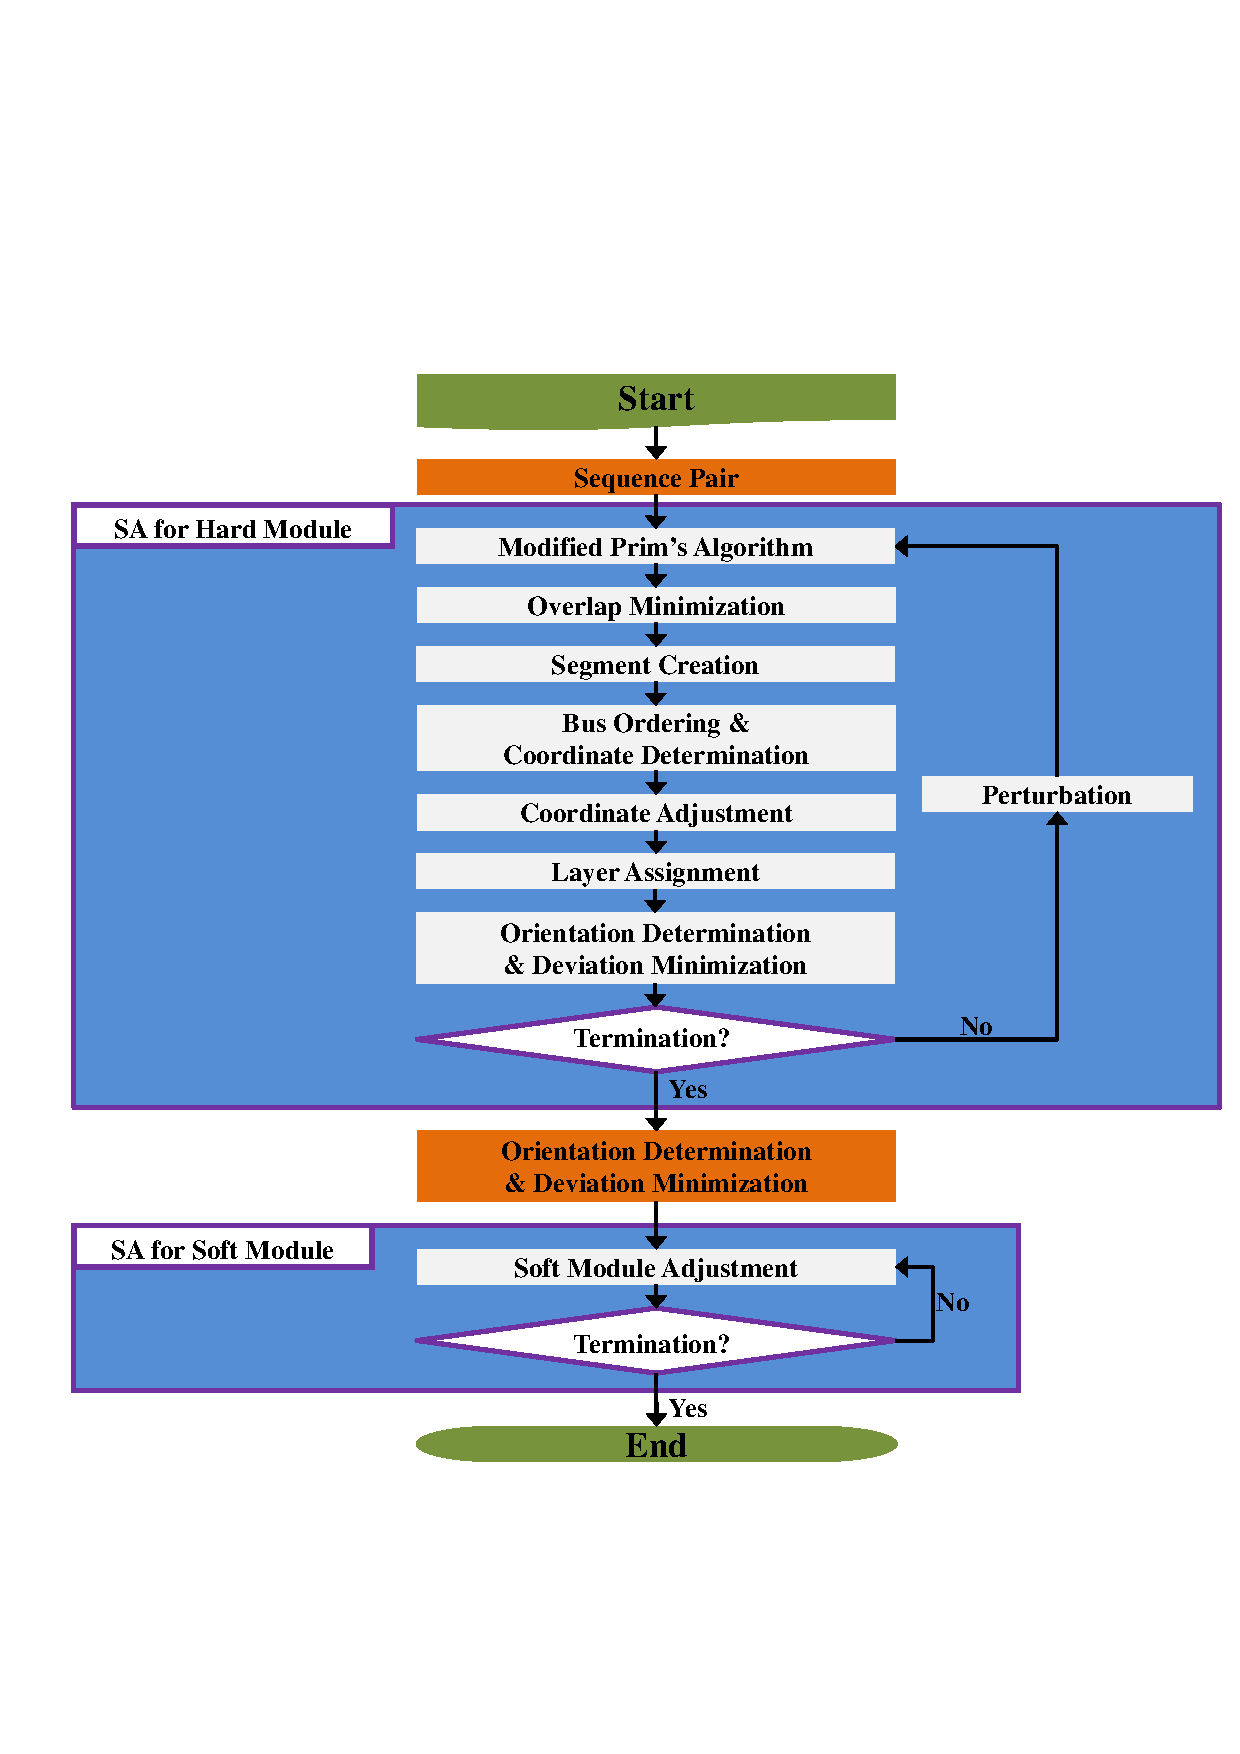
\includegraphics[width=13cm]{Fig/flowchart.pdf}
   %\centerline{\psfig{figure=Fig/flowchart.eps, width=13cm}}
     \caption{
      Algorithm overview.
   }
  \label{fig::flowchart}
\end{figure}

The flowchart of our bus-pin-aware bus-driven floorplanning
algorithm is shown in Figure~\ref{fig::flowchart}.
In the beginning of our algorithm, it derives a floorplan by using
the sequence pair representation \cite{Murata95}, then it computes
the coordinate of each module on the floorplan to obtain the geometric
relations between modules.
Next, the modified Prim's algorithm is used to obtain bus routing topologies,
and it applies the overlap minimization algorithm to minimize the overlap between
different bus components in the MST.
Since some bus pins may not be passed by the buses, it needs to add some buses
for connecting the bus pins to the MST.
After the above steps, several horizontal and vertical buses are obtained,
and their coordinate could be determined. Then, it performs coordinate adjustment algorithm
to further optimize the wirelength by adjusting the coordinate of each bus.
Since extra vias are \textbf{\textit{forbidden}}
at the bend of the diagonal buses, the modified graph coloring algorithm
is used to assign each bus to different layers.
Then the algorithm discussed in the Section~\ref{sec::Fast Deviation Update Based on Topology Comparison}
is used to determine the position and orientation of each bus pin for the current solution, meanwhile, it
minimizes the deviation at each load.

During perturbation, it has three operations to
perturb the current floorplan: (1) Rotate. (2) Reverse. (3) Swap.
The cost function used in this paper is defined as follows:
\begin{eqnarray}
Cost = \alpha \cdot \textbf{\textit{A}} + \beta \cdot
\textbf{\textit{B}} + \gamma \cdot \textbf{\textit{I}}
\end{eqnarray}

where \textbf{\textit{A}} is the chip area, \textbf{\textit{B}} is
the bus area, \textbf{\textit{I}} is the number of invalid bus nets,
$\alpha$, $\beta$, and $\gamma$ are parameters defined by the users.
For saving runtime, it only performs the bus routing algorithm when
the current chip area is smaller than the chip area of the best solution.
Each time a better solution is found, it will check the deviation of
the best solution and the current solution, the solution
with best deviation will be stored.

After the simulated annealing stage, the algorithm discussed in
the Section~\ref{sec::Fast Deviation Update Based on Topology Comparison} is performed to
determine the position and orientation of each bus pin for the best solution. Finally, it changes either the
width or height of the modules lying on the critical path to obtain
a better chip area.

\section{Modified Prim's Algorithm} \label{sec::Modified Prims Algorithm}
To derive the bus topologies, it first constructs the MST for connecting the
bus modules. Since the deviation is calculated from the driver to each load,
to take the impact of the deviation into consideration,
we adopt the Prim's algorithm to construct the MST from
the driver. During constructing the MST, it checks the capacity
of each module to avoid violating capacity constraint. If the selected
edges violate the constraint, then other edges will be chosen to
connect the MST. The bus is regarded as infeasible if no MST is finally
constructed.

\begin{figure}[htb]
  \centering
    \includegraphics[width=8.8cm]{Fig/MST.pdf}
    %\centerline{\psfig{figure=Fig/MST.eps, width=8.8cm}}
     \caption{
       (a) Minimum spanning tree. (b) The resulting routing tree.
   }
  \label{fig::minimum_spanning_tree}
\end{figure}

Figure~\ref{fig::minimum_spanning_tree} (a) is an example of the
MST. The MST connects the modules $m_1$, $m_2$, $m_3$, $m_7$, and
$m_8$, the weight of each edge is derived from the distance
between different modules. For instance, the weight $d_c$ of the diagonal
bus connecting $m_2$ and $m_7$ is $d_1$ + $d_2$. When determining the
coordinate of each bus, it only handles the horizontal and vertical
buses, thus, each diagonal bus in the MST will be split into one
horizontal and one vertical buses.
Figure~\ref{fig::minimum_spanning_tree} (b) shows the routing
result of Figure~\ref{fig::minimum_spanning_tree} (a).

During constructing the MST, it considers the diagonal connection
between different modules, checks the capacity constraint, and
minimizes the bus wirelength. Therefore, we modify the Prim's algorithm to
meet the above requirements.

\section{Segment Creation}
\label{sec::Segment Creation}

\begin{figure}[htb]
  \centering
    \includegraphics[width=8.8cm]{Fig/segment_creation.pdf}
    %\centerline{\psfig{figure=Fig/segment_creation.eps, width=8.8cm}}
     \caption{
      \small
       (a) Before adding segment. (b) After adding segment.
   }
  \label{fig::segment_creation}
\end{figure}

During constructing the MST, the position of the bus pins is ignored,
as a result, the bus pin of some modules may not be passed by the MST.
To connect the bus pin to the MST, some segments must be added to meet the
requirement. Figure~\ref{fig::segment_creation} (a) is an example, the bus connects four modules $m_1$,
$m_4$, $m_5$, and $m_7$, and the bus pin on module $m_5$ is not passed by the MST.
To solve this problem, one horizontal segment is added for connecting the bus pin on the module $m_5$ to the MST.
The result of segment addition is shown in Figure~\ref{fig::segment_creation} (b).

\section{Bus Ordering and Coordinate Determination}
\label{sec::Bus Ordering and Coordinate Determination}
\subsection{Bus Ordering} \label{sec::Bus Ordering}
Since the coordinate of each bus is determined in non-decreasing
order, it finds the bus ordering of all horizontal (vertical)
buses and determines the coordinate of each bus according to the
bus ordering \cite{Xiang03}. Given a sequence pair, it can obtain the relative
position of any two modules, and the ordering of any two buses is
derived from the relative position of those modules passed by the
buses.

\begin{figure}[htb]
  \centering
    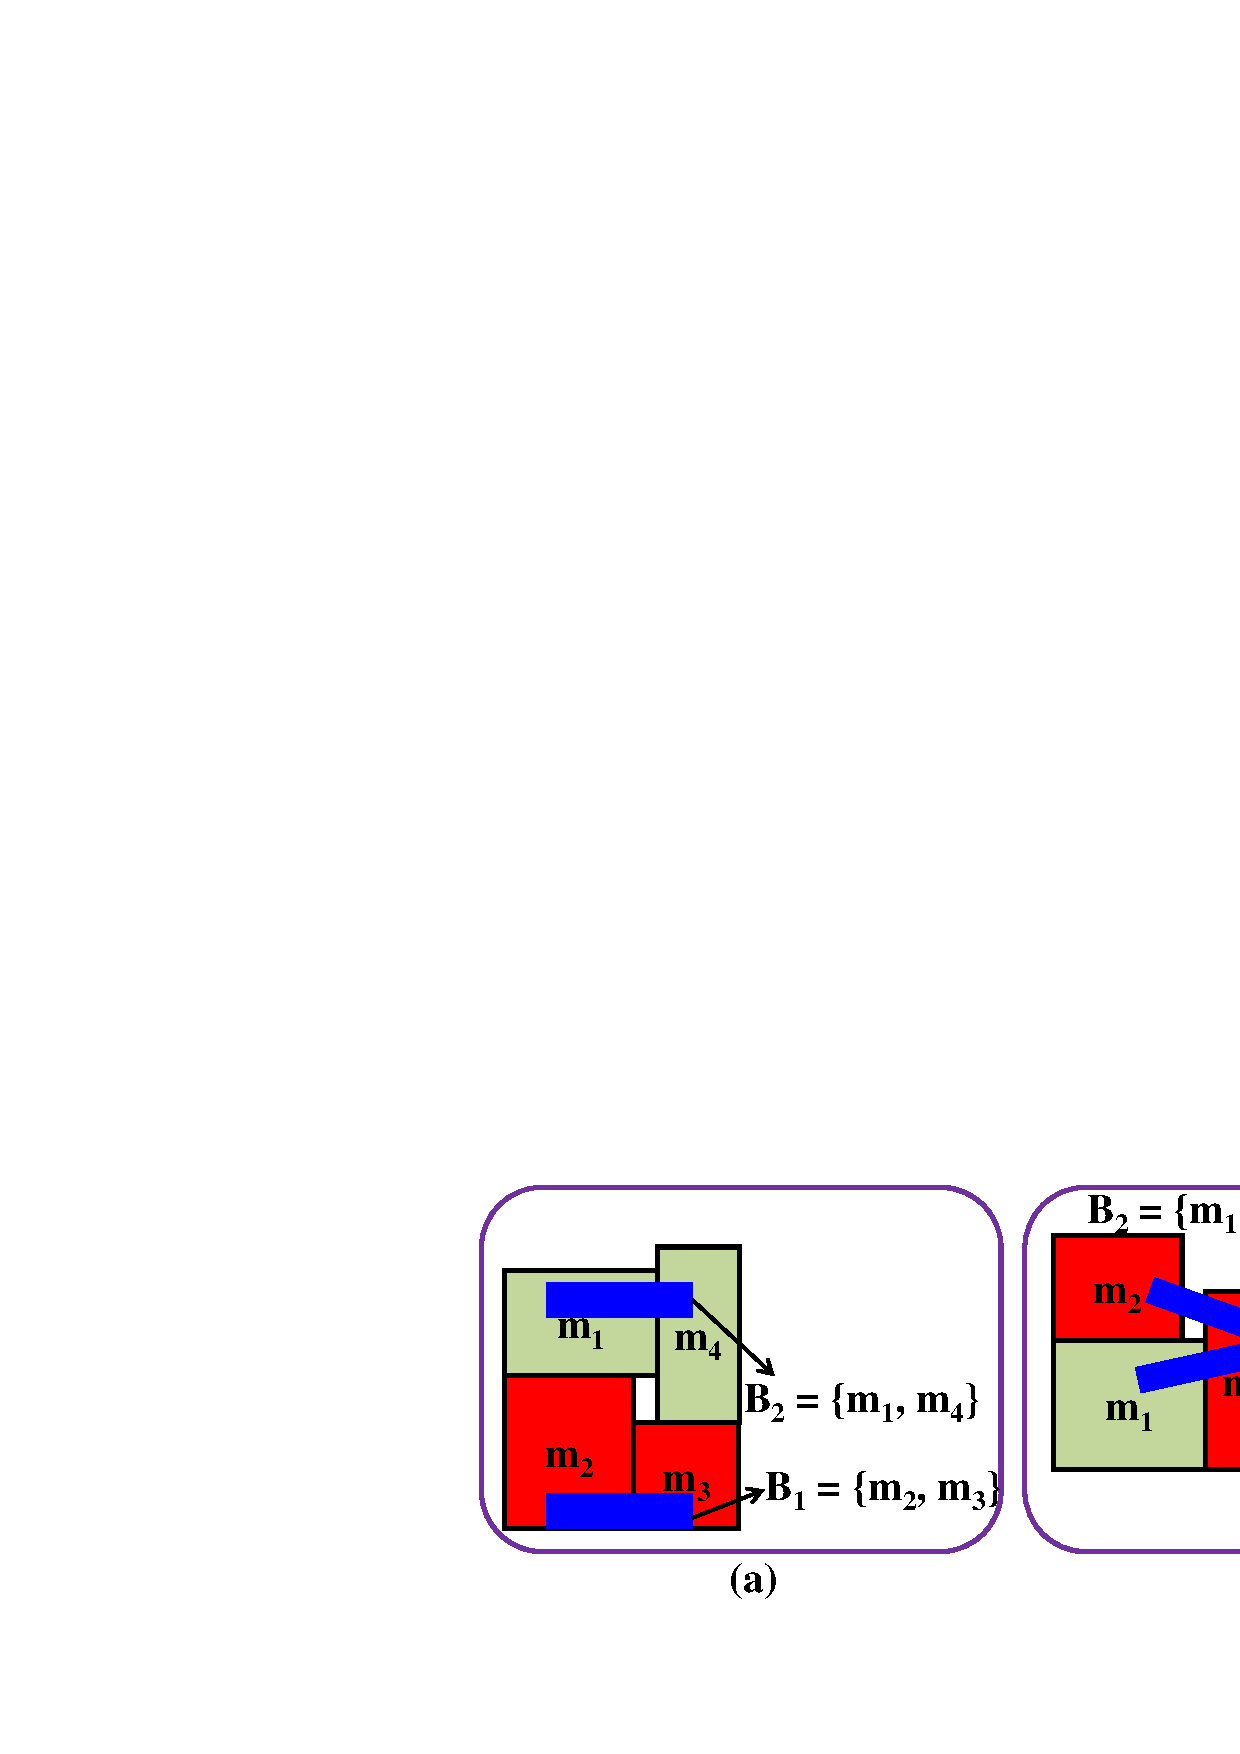
\includegraphics[width=12cm]{Fig/bus_ordering.pdf}
    %\centerline{\psfig{figure=Fig/bus_ordering.eps, width=12cm}}
     \caption{
       (a) Bus ordering. (b) Bus crossing. (c) Ordering constraint graph.
   }
  \label{fig::bus_ordering}
\end{figure}

Figure~\ref{fig::bus_ordering} (a) gives an example. The sequence
pair of the floorplan is (1243, 2314), two buses $B_1$ = \{$m_2$,
$m_3$\} and $B_2$ = \{$m_1$, $m_4$\} are placed on the floorplan.
The module $m_1$ is placed above the module $m_2$ according to the
sequence pair, thus, the bus $B_2$ passing through the module
$m_1$ has to be placed above the bus $B_1$ passing through the
module $m_2$. This condition is called $bus\ ordering$.
In order to obtain the bus ordering between any two buses, it
constructs the ordering constraint graph (OCG) by performing the
above steps on any two horizontal (vertical) buses. The buses are
represented as the nodes in the OCG, and the edges represent the
ordering between any two buses.

During determining the bus ordering, different buses may conflict
with each other. In Figure~\ref{fig::bus_ordering} (b), two buses
$B_1$ = \{$m_2$, $m_3$, $m_5$\} and $B_2$ = \{$m_1$, $m_4$,
$m_6$\} are placed on the floorplan. Based on the sequence
pair, the module $m_2$ is placed above the module $m_1$, and the
module $m_6$ is placed above the module $m_5$. Since the modules
$m_1$ and $m_2$ are passed by the buses $B_2$ and $B_1$,
respectively, an edge from the node $B_1$ to the node $B_2$ is
inserted into the OCG. Besides, the modules $m_5$ and $m_6$
are passed by the buses $B_1$ and $B_2$, respectively, an edge
from node $B_2$ to node $B_1$ is inserted into the OCG. Thus, the OCG
contains a cycle as shown in Figure~\ref{fig::bus_ordering} (c).
It means that two buses conflict with each other, and one of the
two buses is regarded as infeasible. This situation is called
$bus\ crossing$.

To determine the bus ordering of all horizontal (vertical) buses
from the OCG, we first set the nodes with zero out-degree in the
OCG the highest priority comparing with remaining horizontal
(vertical) buses. By this property, it determines the bus ordering
by deleting the nodes and edges from the OCG iteratively. In each
iteration, it removes the node with zero out-degree and deletes
the edges connecting to it from the OCG. If no such node in the
OCG, it means that the cycle is contained in the OCG and one of the
minimum out-degree nodes is regarded as infeasible. Then the
invalid node and the edges connecting to it will be deleted from
the OCG. The above steps are repeated until all nodes are removed
from the OCG. Finally, the bus ordering of all feasible horizontal
(vertical) buses can be obtained.
\subsection{Coordinate Determination}
\label{sec::Coordinate Determination} After determining the bus ordering, it
starts to determine the coordinate of all horizontal (vertical)
buses \cite{Xiang03}. Without loss of generality, we take the horizontal buses
for example. The coordinate of each horizontal bus $B_i$ is
$y_{max}$ = max\{$y_i$ $|$ $i$ = 1, 2, ..., k\}, where k is the
number of the modules passed by the bus, and $y_i$ is the y
coordinate of each module. If some modules are not passed by the bus $B_i$.
It adjusts the coordinate of each module slightly
such that all modules can be passed by the bus $B_i$.

 \begin{figure}[htb]
  \centering
    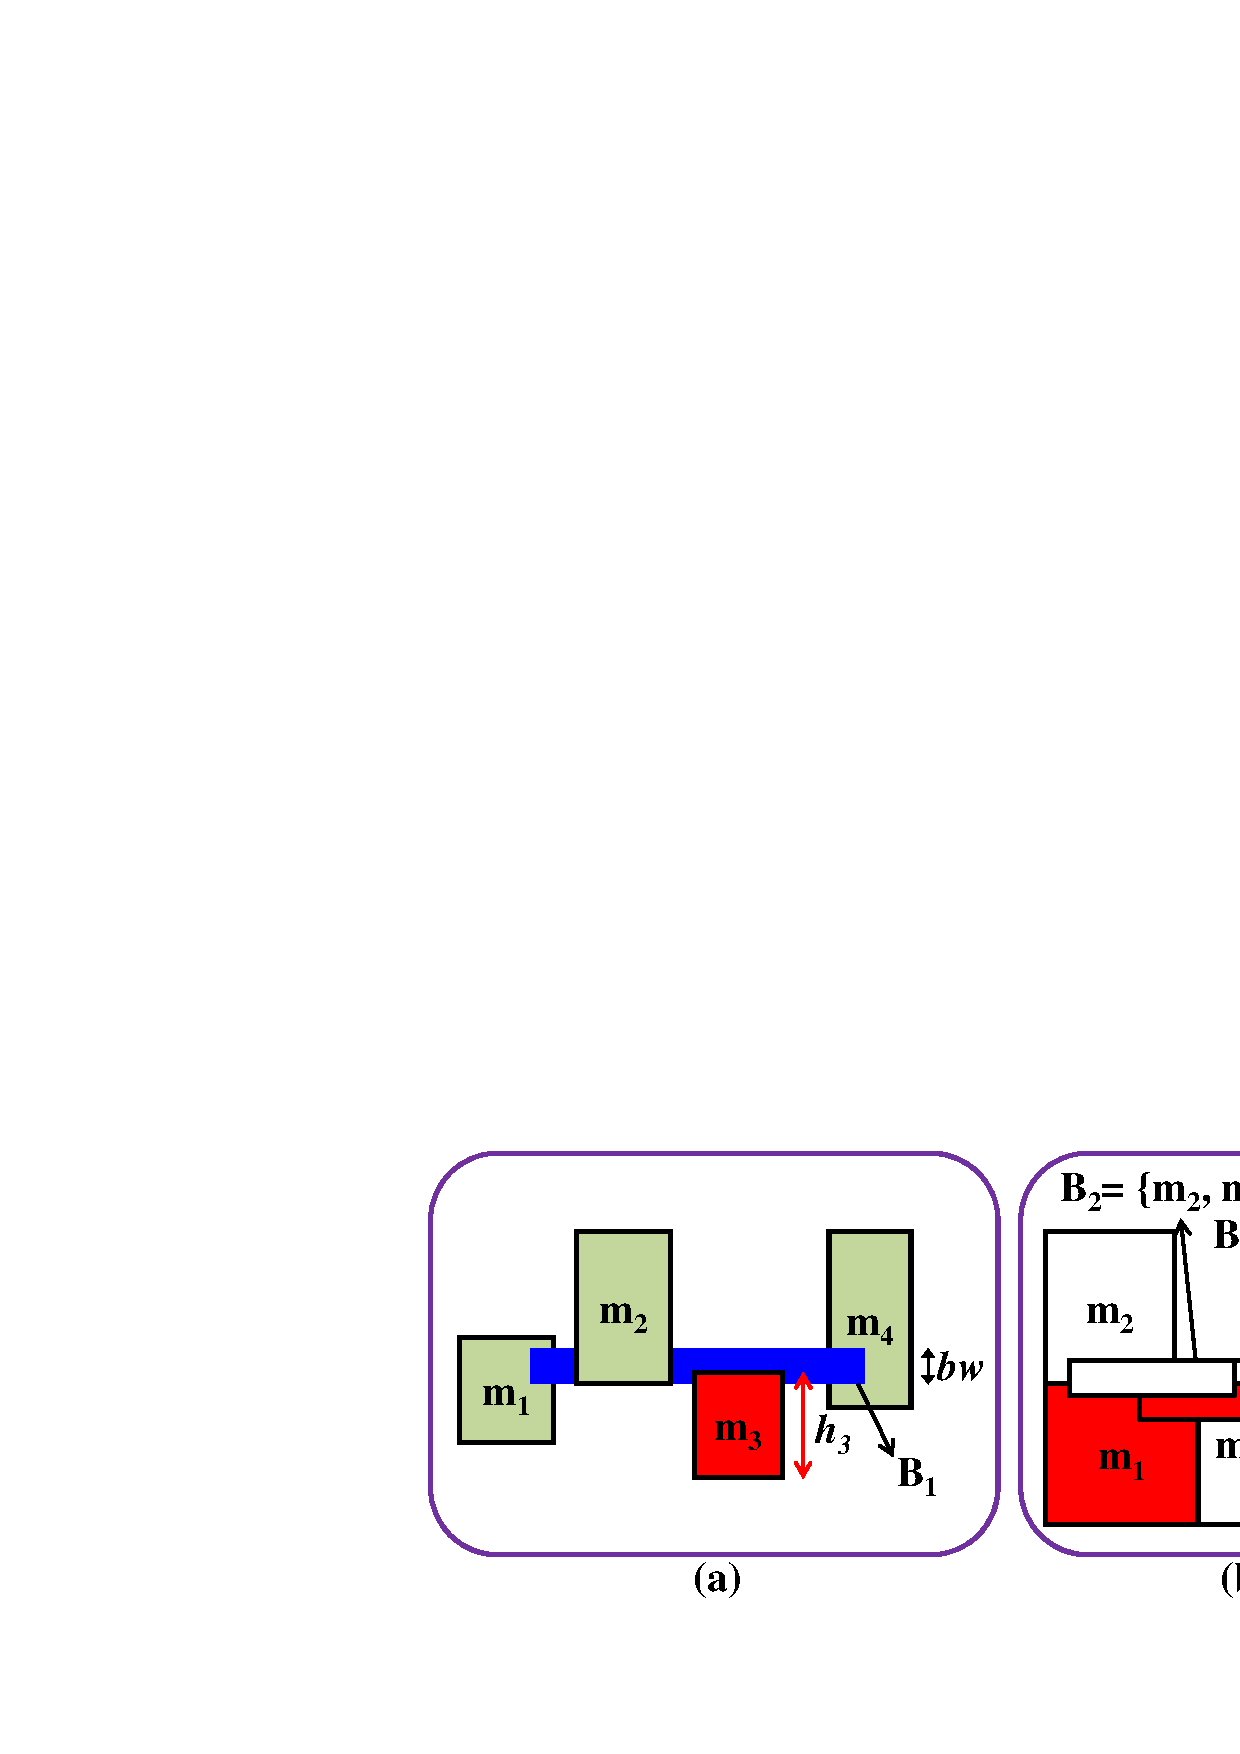
\includegraphics[width=12cm]{Fig/bus_overlapping.pdf}
    %\centerline{\psfig{figure=Fig/bus_overlapping.eps, width=12cm}}
     \caption{
       (a) Module moving. (b) Bus overlapping. (c) No bus overlapping.
   }
  \label{fig::bus_overlapping}
\end{figure}

In Figure~\ref{fig::bus_overlapping} (a), the bus $B_1$ goes
through the modules in \{$m_1$, $m_2$, $m_3$, $m_4$\}, the bus
width of $B_1$ is $bw$, the height of the module $m_i$ is $h_i$.
In this figure, the coordinate of $B_1$ is $y_{max}$ = max\{$y_i$
$|$ $i$ = 1, 2, 3, 4\}. Since the module $m_3$ is not passed by the
bus $B_1$, it changes the coordinate of the module $m_3$
slightly such that it can be passed by $B_1$, the new coordinate
of $m_3$ is $y_{max}$ + $bw$ - $h_3$.

When considering multiple horizontal (vertical) buses, different
horizontal (vertical) buses may overlap with each other. In
Figure~\ref{fig::bus_overlapping} (b), the buses $B_1$ = \{$m_1$,
$m_5$\} and $B_2$ = \{$m_2$, $m_3$\} are placed on the floorplan.
The bus $B_2$ overlaps with the bus $B_1$ on the floorplan, this
situation is called $bus\ overlapping$. Therefore, the bus $B_2$ has
to be moved up until there is no overlap with the buses below. The result is shown in
Figure~\ref{fig::bus_overlapping} (c).

\section{Wirelength Reduction}
\subsection{Overlap Minimization}
\label{sec::Overlap Minimization}
Since the width and height of each module is not considered during constructing the MST,
the bus wirelength may be further optimized. In this paper,
we propose an algorithm to reduce the overlap in MST such that
the better bus wirelength could be obtained.

\begin{figure}[htb]
  \centering
    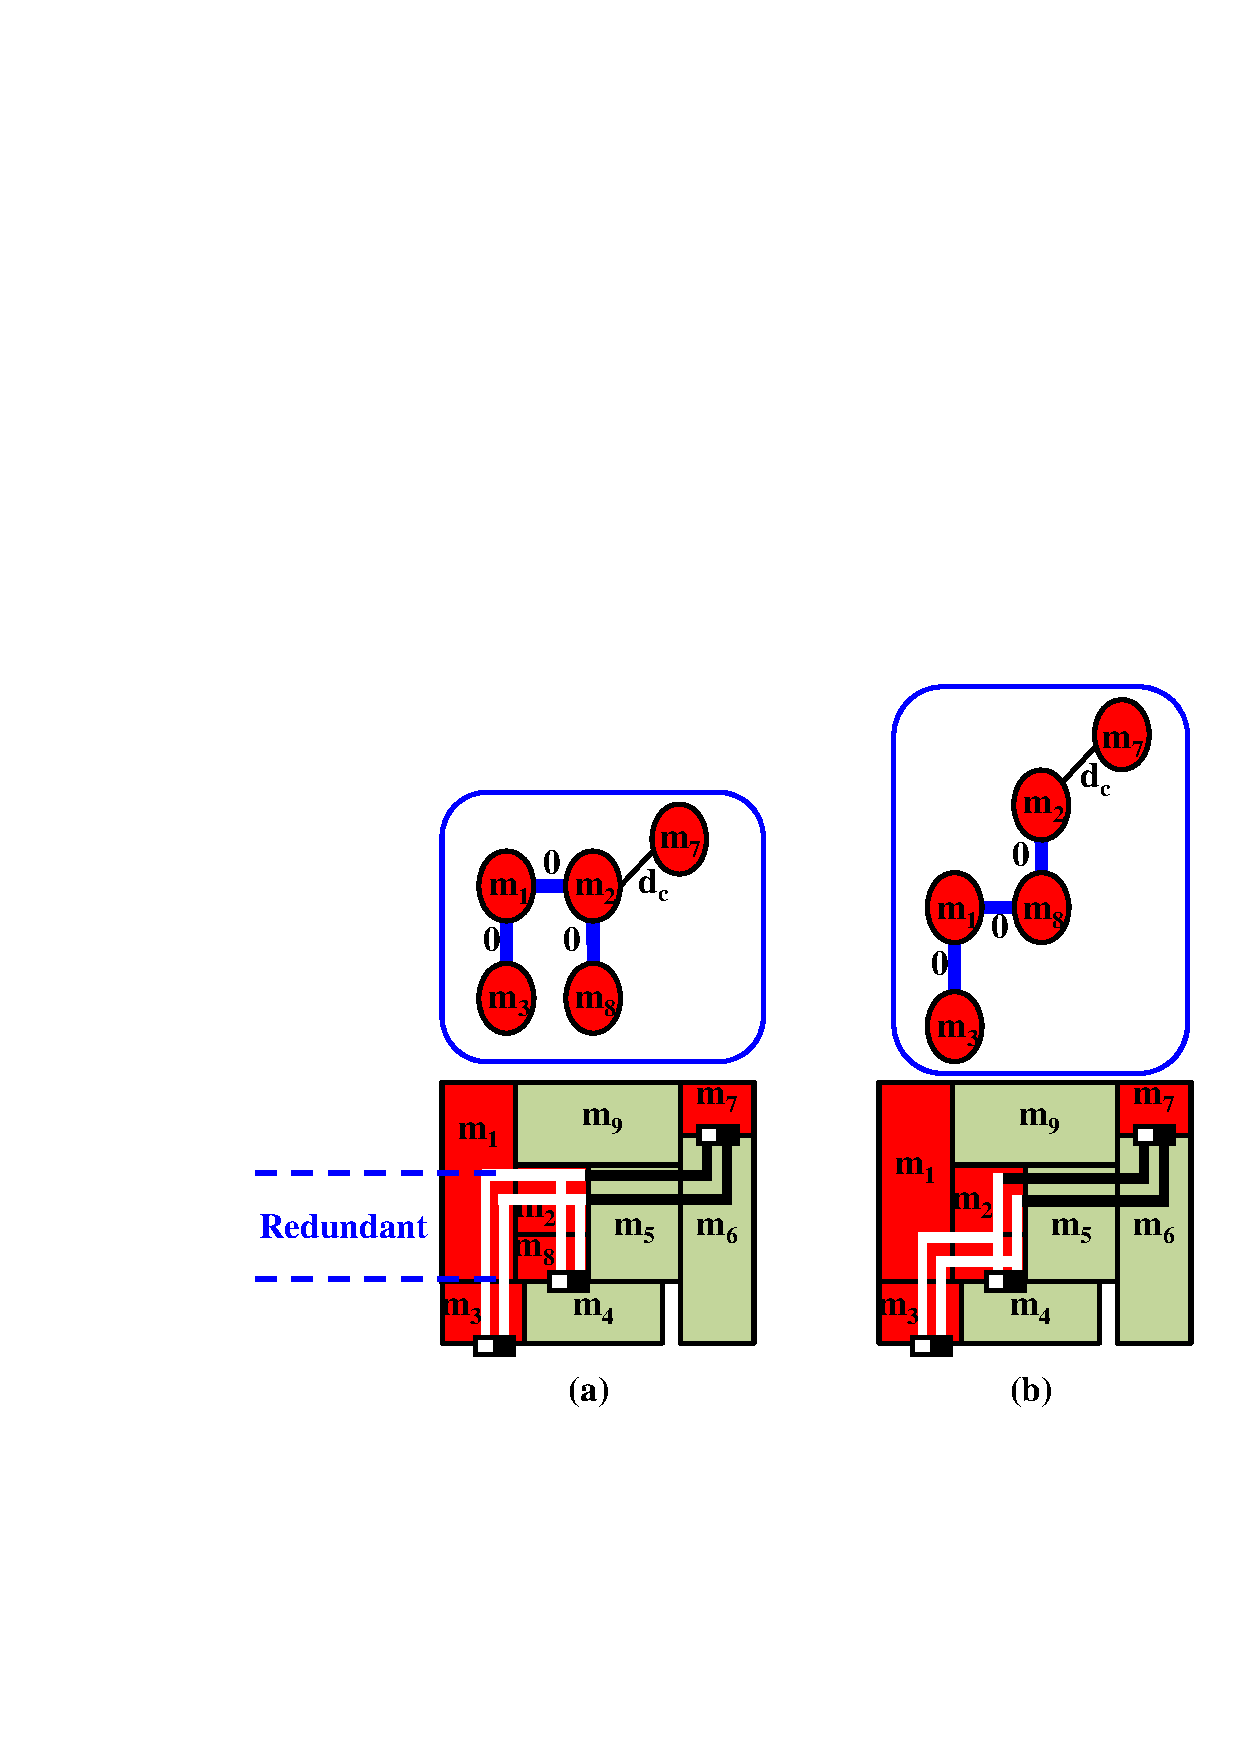
\includegraphics[width=11cm]{Fig/overlap_minimization.pdf}
    %\centerline{\psfig{figure=Fig/overlap_minimization.eps, width=11cm}}
     \caption{
      \small
       (a) Before wirelength reduction. (b) After wirelength reduction.
   }
  \label{fig::overlap_minimization}
\end{figure}

Figure~\ref{fig::overlap_minimization} illustrates how
the algorithm works. The bus connects the five modules $m_1$,
$m_2$, $m_3$, $m_7$, and $m_8$. In Figure~\ref{fig::overlap_minimization} (a),
there are three bus components which form the U-shaped pattern --- one vertical bus component
connects modules $m_1$ and $m_3$, another vertical bus component connects
modules $m_2$ and $m_8$, and the horizontal bus component connects modules
$m_1$ and $m_2$. If the overlap in the U-shaped pattern can be minimized, then
total bus wirelength can be further optimized.
Thus, the horizontal bus component is shifted down to minimize the overlap between the buses.
Figure~\ref{fig::overlap_minimization} (b) demonstrates the
result of wirelength reduction. All the above steps are repeated until all horizontal and vertical
bus components are searched.

\begin{Lemma}
Minimize the overlap in the obtained MST will further decrease the
total bus wirelength of the MST.
\end{Lemma}

\begin{figure}[htb]
  \centering
    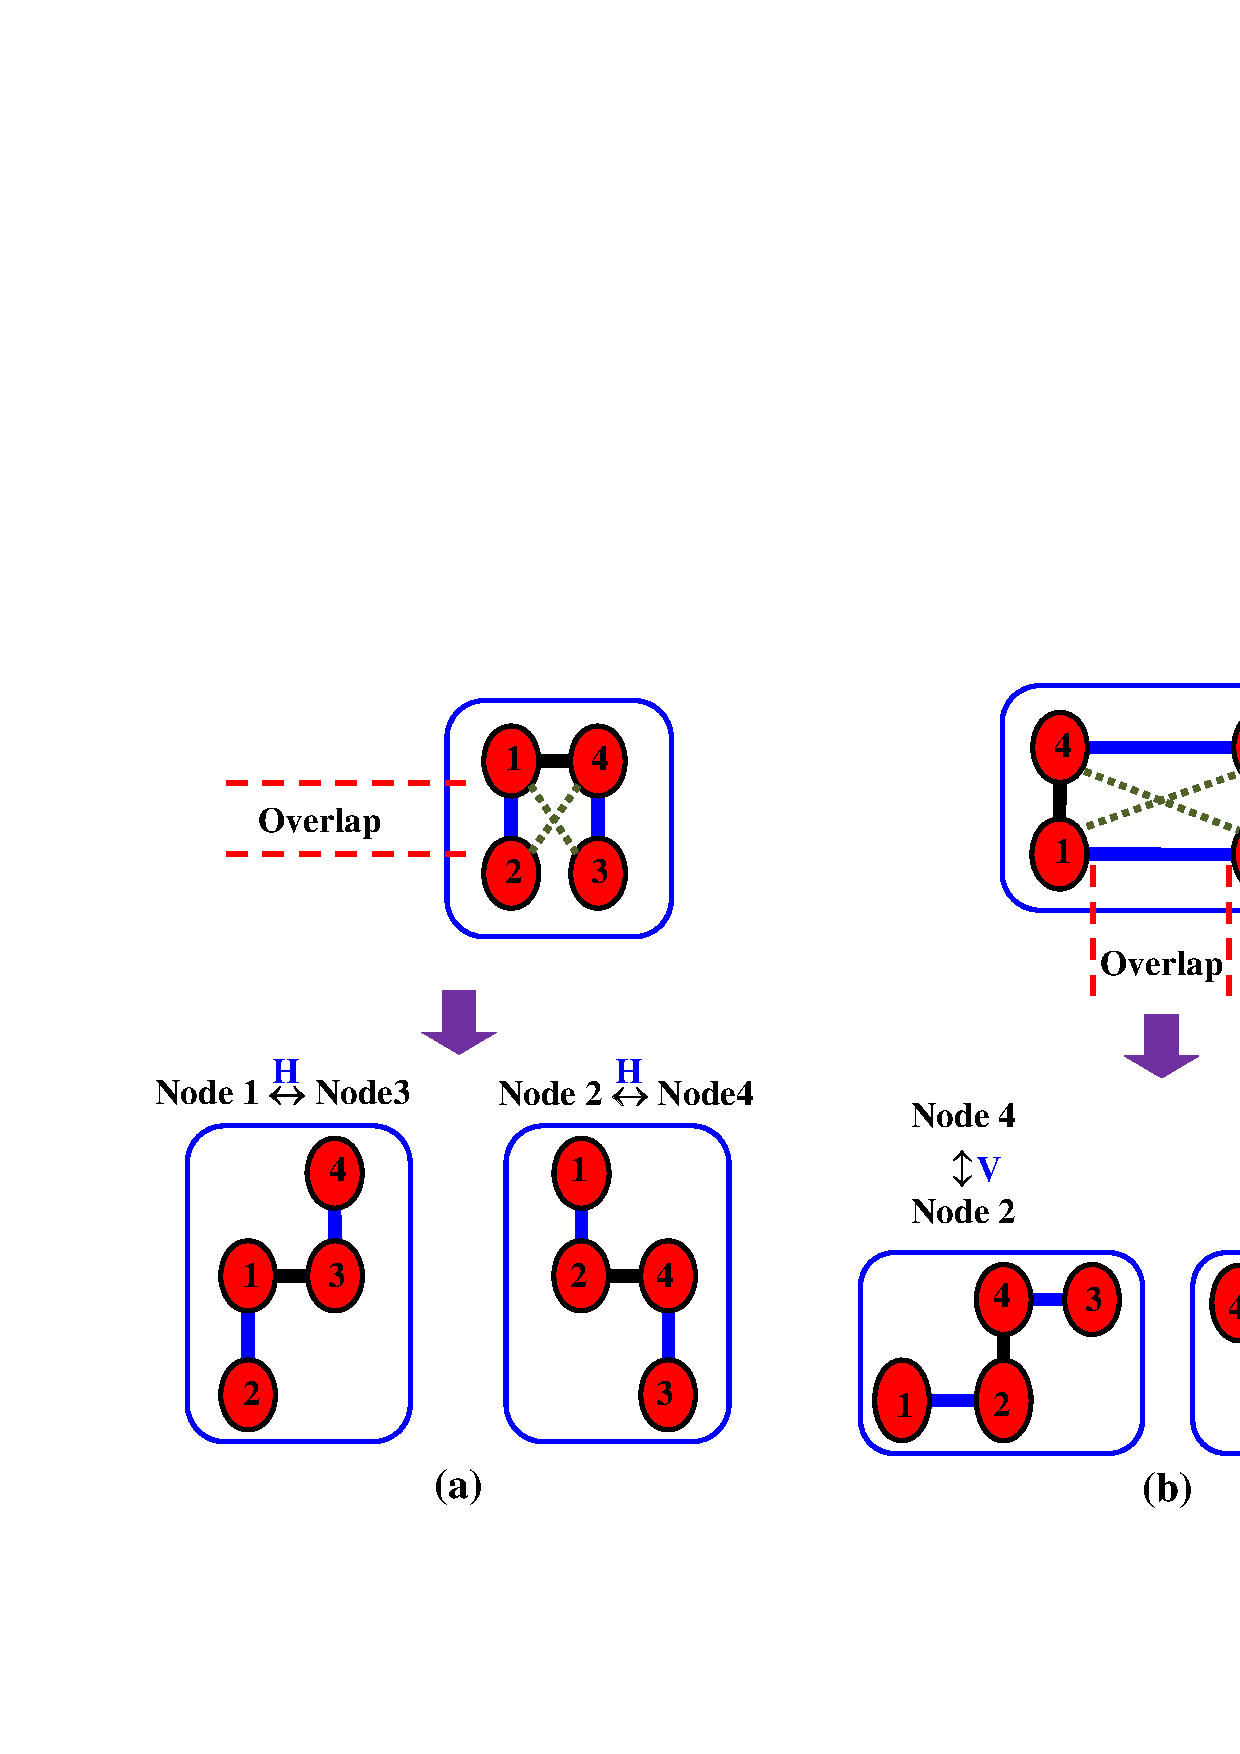
\includegraphics[width=12cm]{Fig/lemma1.pdf}
    %\centerline{\psfig{figure=Fig/lemma1.eps, width=12cm}}
     \caption{
      \small
       (a) Reduction rule for horizontal bus components. (b) Reduction rule for vertical bus components.
   }
  \label{fig::lemma1}
\end{figure}

During constructing the MST for each bus, it ignores the actual information
on the width and height of the module, as a result, the wirelength of the obtained MST may
be further optimized.
For each bus, it will construct a MST.
In each MST, the bus modules are represented as the nodes, and the bus components are represented as the edges.
If one MST contains the U-shaped bus pattern, it means that
there is a overlap in the MST. Therefore, the bus wirelength can be minimized by minimizing the overlap in the MST.

Figure~\ref{fig::lemma1} shows the reduction rule.
In Figure~\ref{fig::lemma1} (a), it shows the reduction rule for the horizontal bus components.
Each time a matched U-shaped patten is found, it will check either
the node 1 is horizontal with the node 3 or the node 2 is horizontal with the node 4.
If the node 1 is horizontal with node 3, then the horizontal bus component connecting
the node 1 and 4 is changed to connect the node 1 and node 3.
If the node 2 is horizontal with node 4, then the horizontal bus component connecting
the node 1 and 4 is changed to connect the node 2 and node 4.
Then, the overlap is minimized to improve the bus wirelength.
Figure~\ref{fig::lemma1} (b) shows the reduction rule for the vertical bus components.
The rule can be derived similarly.

\subsection{Coordinate Adjustment}
\label{sec::Coordinate Adjustment}
When determining the coordinate of each bus, it only focuses on
making each horizontal (vertical) buses feasible but not on
minimizing the bus wirelength. However, different coordinates of
each bus result in different interconnect wirelength
between the horizontal and vertical bus components.
Therefore, the bus wirelength can be further optimized
by properly adjusting the coordinate of each bus component.

\begin{figure}[htb]
  \centering
    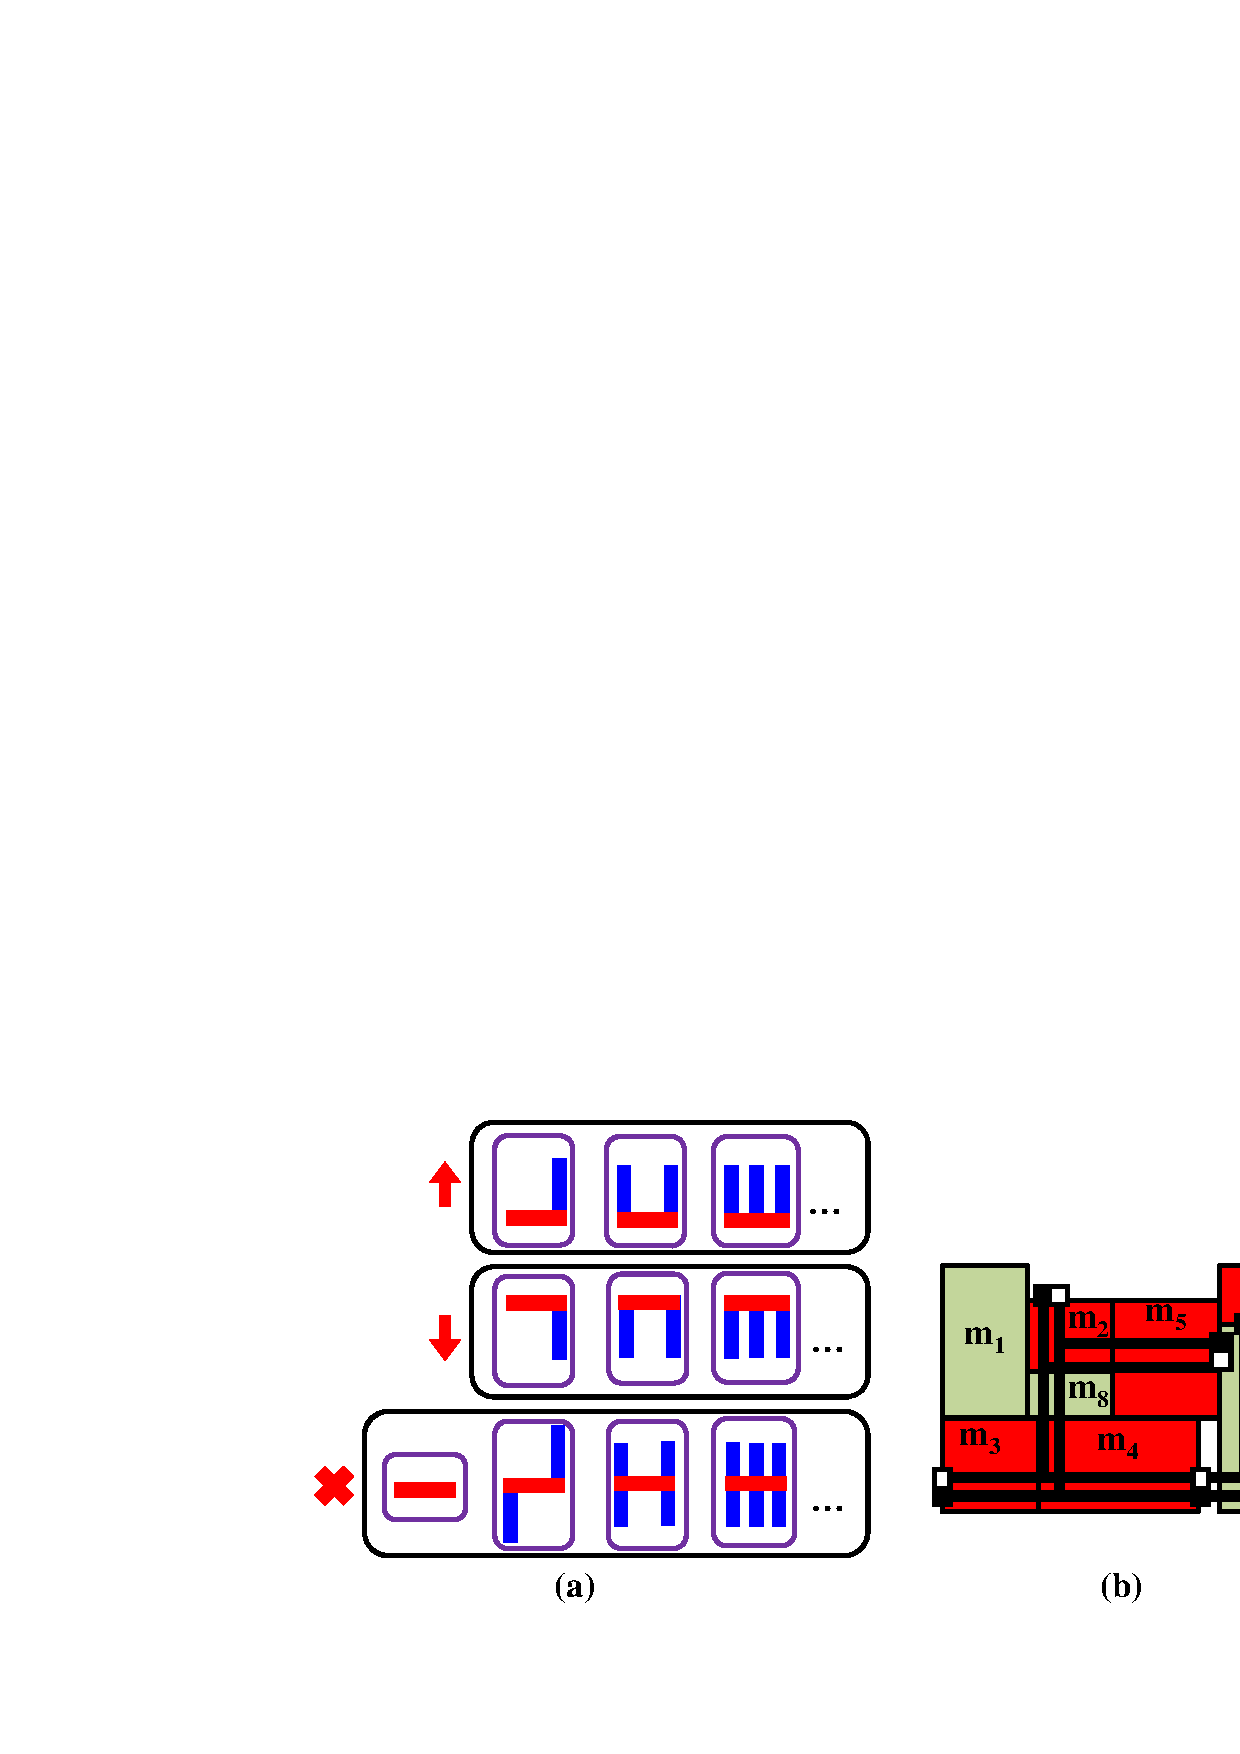
\includegraphics[width=14cm]{Fig/coordinate_adjustment.pdf}
    %\centerline{\psfig{figure=Fig/coordinate_adjustment.eps, width=14cm}}
     \caption{
       (a) Wirelength reduction rule. (b) Before wirelength reduction. (c) After wirelength reduction.
   }
  \label{fig::coordinate_adjustment}
\end{figure}

Figure~\ref{fig::coordinate_adjustment}
(a) illustrates how it works, the horizontal bus component is the target to
be reduced the interconnect wirelength. In the first row, the number of the
vertical bus components intersecting with the horizontal bus component in upper side are
more than in lower side. Thus, it moves the horizontal bus component toward
the upper side to improve its wirelength. In the second row, the
number of the vertical bus components intersecting with the horizontal bus component in
lower side are more than in upper side. Thus, it moves the
horizontal bus component toward the lower side to improve its wirelength. In
the third row, the number of the vertical bus components intersecting with the
horizontal bus component are equal on both side, thus, the coordinate of the horizontal
bus component is not changed.

In Figure~\ref{fig::coordinate_adjustment} (b), the bus = \{$m_2$, $m_3$, $m_4$, $m_5$, $m_7$\}
is placed on the floorplan. Assume we first checks the horizontal bus \{$m_3$, $m_4$\}.
According to the rule as shown in Figure~\ref{fig::coordinate_adjustment} (a), it reduces the wirelength by
moving the bus toward the upper side of the floorplan. The above steps are repeated until all horizontal
and vertical buses are applied, the optimized result is demonstrated in Figure~\ref{fig::coordinate_adjustment} (c).

\begin{Lemma}
Under some specific bus topologies, different positions of each horizontal (vertical) bus
would result in different bus wirelength.
\end{Lemma}

As mentioned earlier, the coordinate of each horizontal bus component is assigned to the highest y-coordinate
of all connected bus modules, and the coordinate of each vertical bus component is assigned to the highest
x-coordinate of all connected bus modules. However, different coordinate of the bus components
result in different interconnect wirelength between the horizontal and vertical bus components.
If the coordinate of each bus component is not carefully assigned,
then the total bus wirelength will be increased dramatically. Nevertheless,
the task is more complicated if it determines the best position of all
horizontal (vertical) bus components simultaneously. Therefore, a better approach is to
decide an initial position for each horizontal (vertical) bus component, then it adjusts
the coordinate of each bus component such that the better bus wirelength can be achieved.

\begin{figure}[htb]
  \centering
    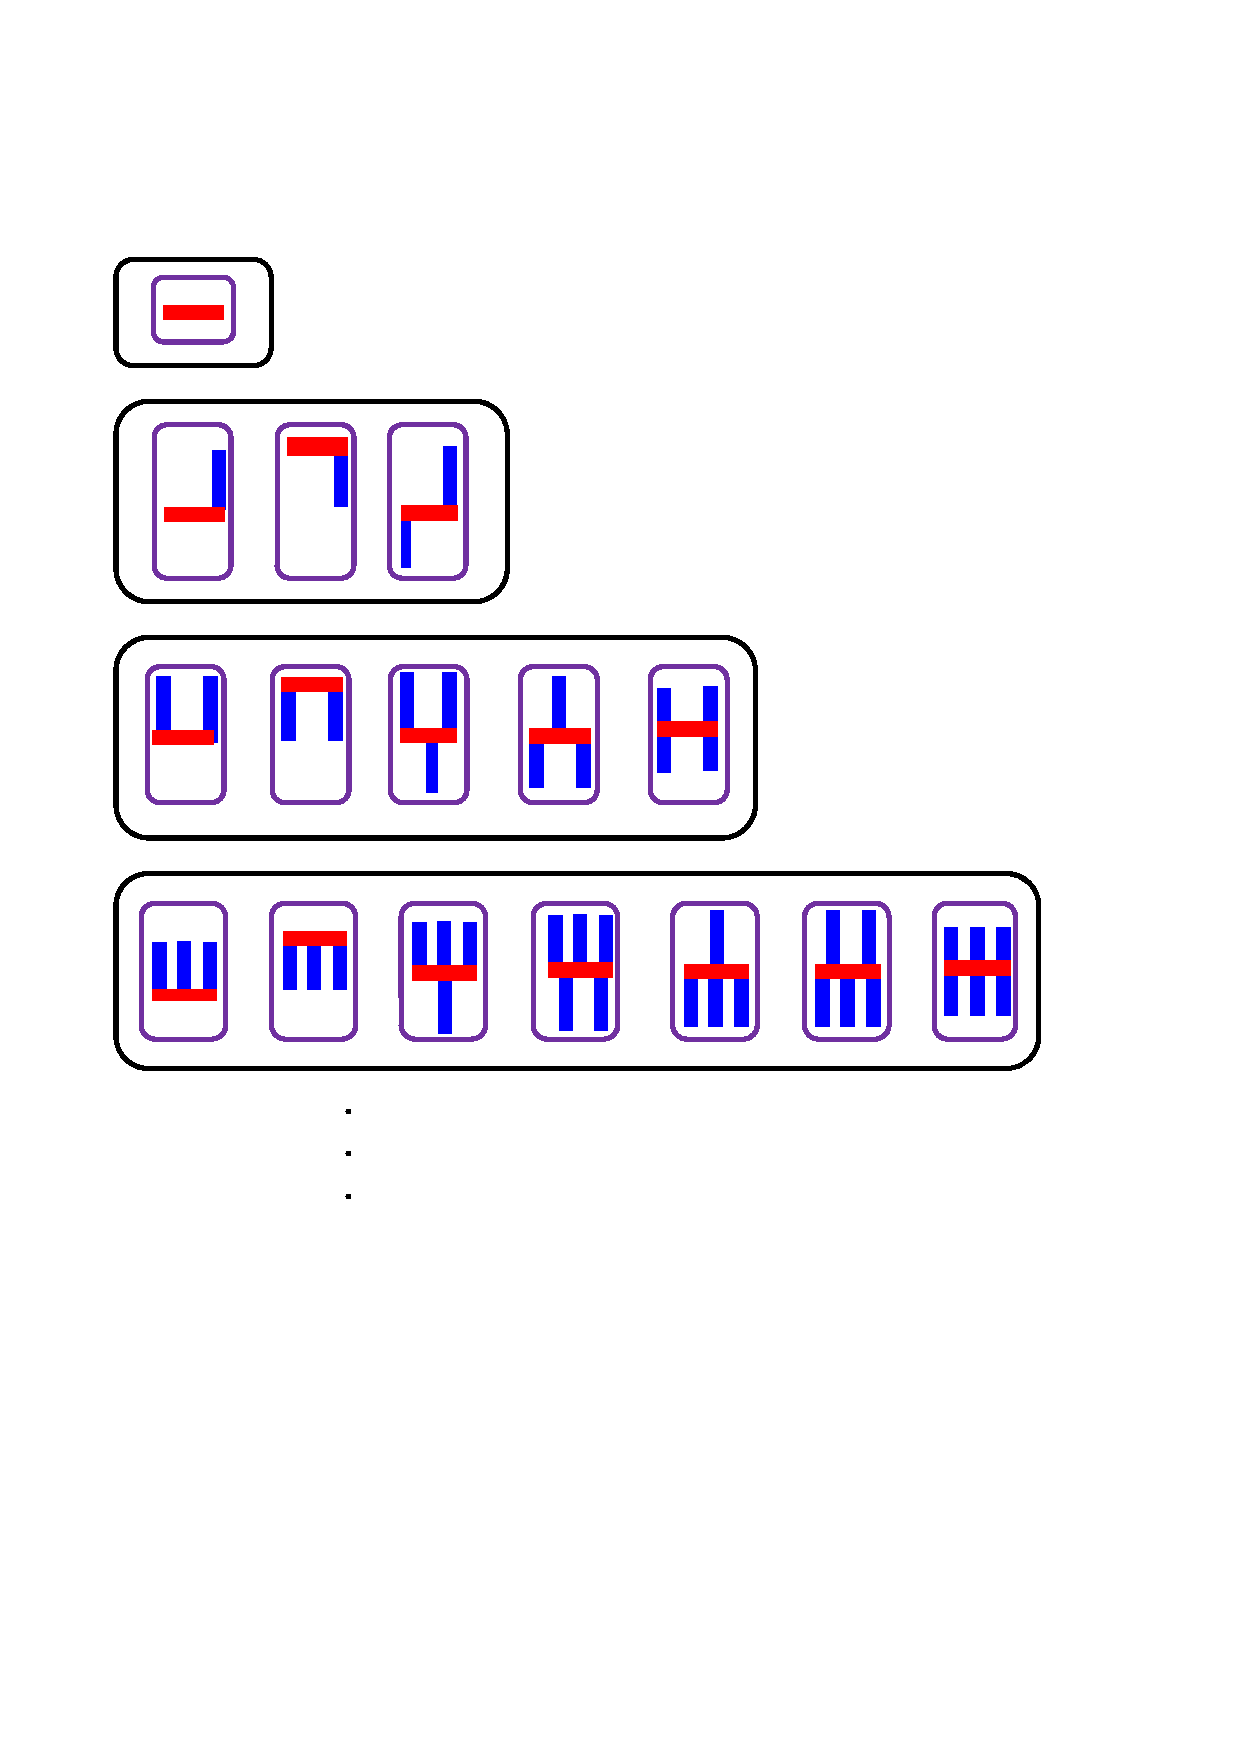
\includegraphics[width=11cm]{Fig/lemma2_1.pdf}
    %\centerline{\psfig{figure=Fig/lemma2_1.eps, width=11cm}}
     \caption{
      \small
       The original bus topology.
   }
  \label{fig::lemma2_1}
\end{figure}

\begin{figure}[htb]
  \centering
    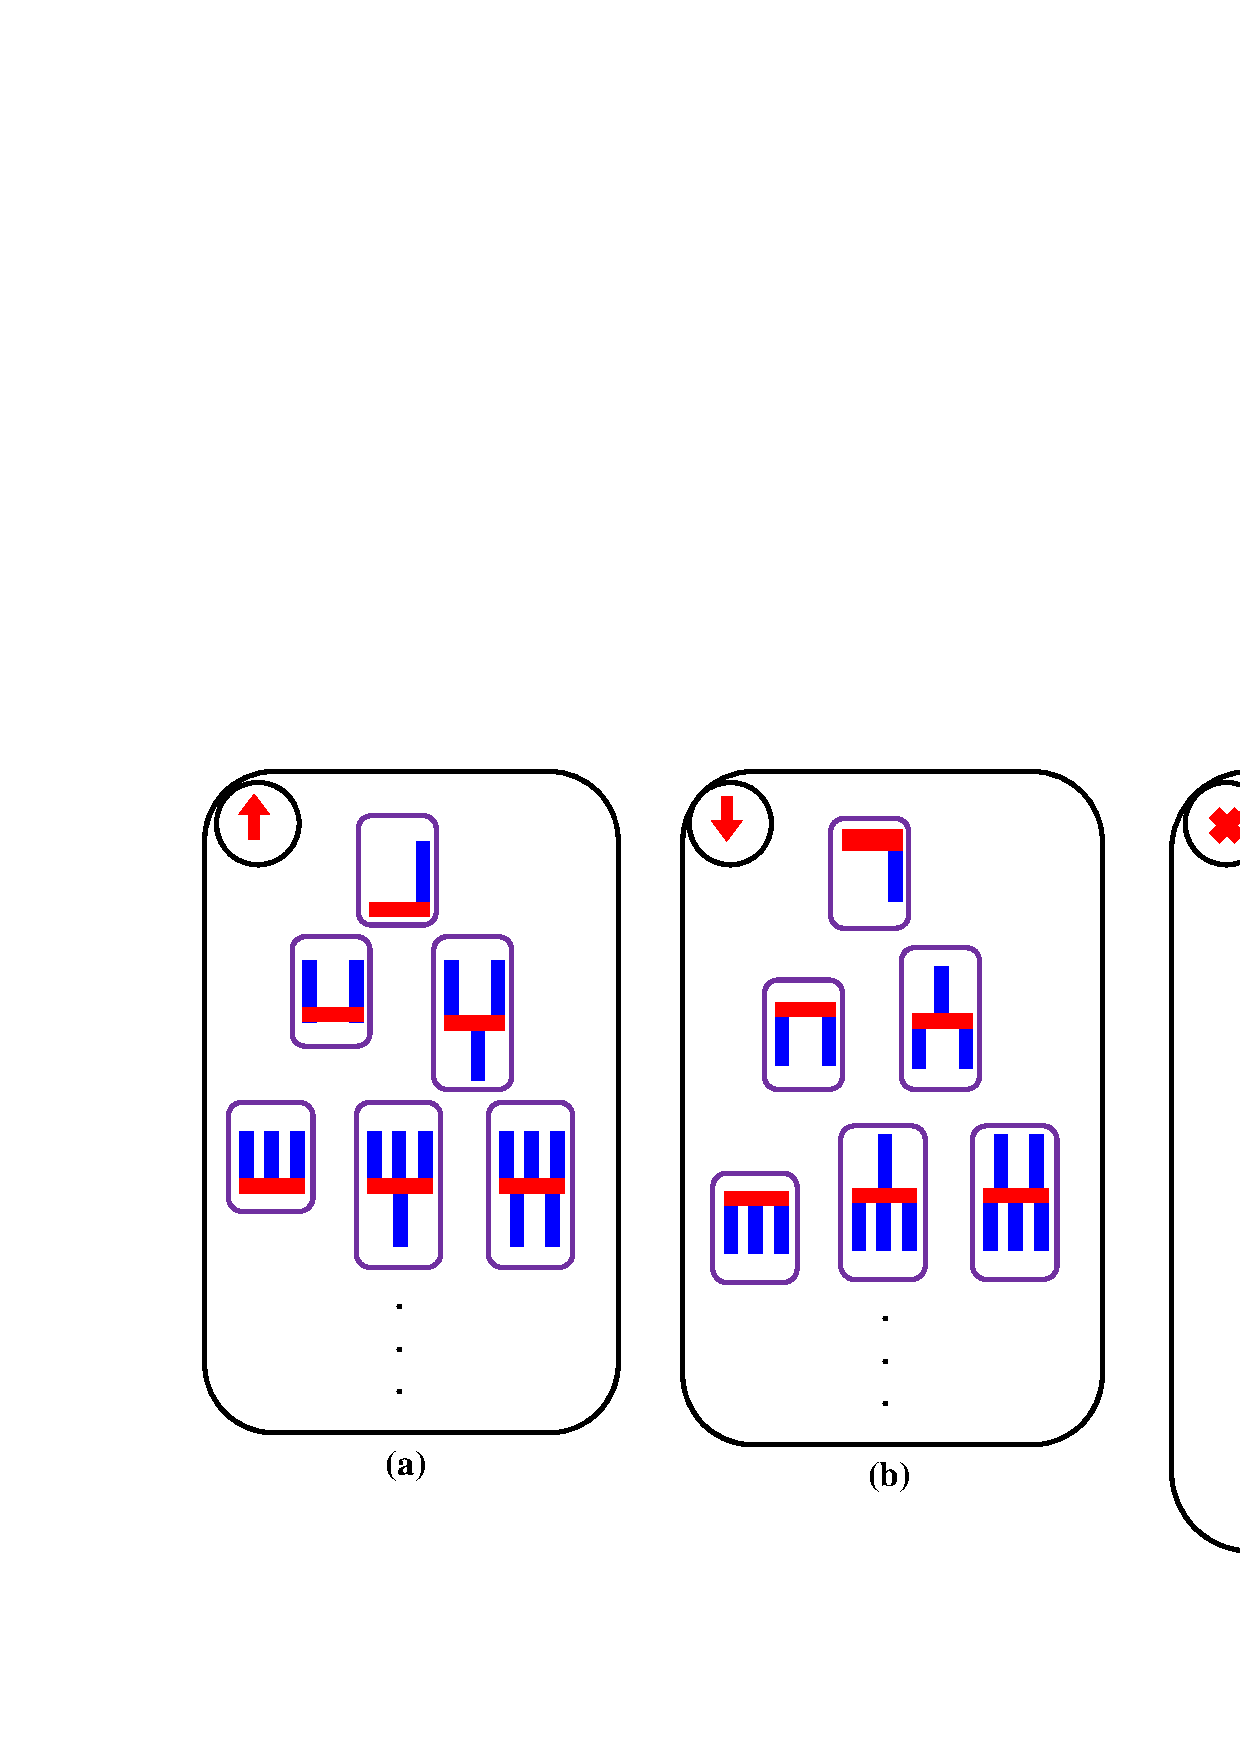
\includegraphics[width=14cm]{Fig/lemma2_2.pdf}
    %\centerline{\psfig{figure=Fig/lemma2_2.eps, width=14cm}}
     \caption{
      \small
       The rules for wirelength reduction.
   }
  \label{fig::lemma2_2}
\end{figure}

Figure~\ref{fig::lemma2_1} and Figure~\ref{fig::lemma2_2} illustrate how to modify the coordinate of each bus component.
In this paper, we explore all possible connective situations between different horizontal and vertical
bus components, parts of the possible connective situations are shown in Figure~\ref{fig::lemma2_1}. In the first row,
there is no any vertical bus components intersecting with the horizontal bus component on both sides.
In the second row, one vertical bus component intersects with the horizontal bus component on one side and one
vertical bus component at most intersects with the horizontal bus component on the other side.
In the third row, two vertical bus components intersect with the horizontal bus component on one side and two
vertical bus components at most intersect with the horizontal bus component on the other side,
the possible situations in other rows can be derived similarly.
All the above situations in Figure~\ref{fig::lemma2_1} can be categorized into three cases as follows:\\
\indent $Case1$: the number of intersecting vertical bus components on upper side of the horizontal bus component
are more than on lower side as shown in Figure~\ref{fig::lemma2_2} (a), thus, the total bus wirelength
will be improved by moving the horizontal bus component toward the upper side.\\
\indent $Case2$: the number of intersecting vertical bus components on lower side of the horizontal bus component
are more than on upper side as shown in Figure~\ref{fig::lemma2_2} (b), thus, the total bus wirelength
will be optimized by moving the horizontal bus component toward the lower side.\\
\indent $Case3$: the number of intersecting vertical bus components are equal on both sides of the horizontal bus component
as shown in Figure~\ref{fig::lemma2_2} (c). No matter how the coordinate of the horizontal bus component is adjusted,
the total bus wirelength remains unchanged.\\

Therefore, each time one horizontal bus component is given, the best bus position can be determined by the
intersecting condition between the horizontal and vertical bus components. For any vertical bus components, the rule can be derived similarly.

\section{Layer Assignment} \label{sec::Layer Assignment}
In this paper, we explore the diagonal connection
that makes the bus shape more flexible to increase the success rate.
Since extra vias are \textbf{\textit{forbidden}} at the bend of the diagonal
buses, we develop an algorithm based on the graph coloring
algorithm to assign the components of the diagonal buses to the
same layer. However, graph coloring is computationally hard. It is
an NP-complete problem if a given graph admits a k-coloring for k
$>=$ 3. In our formulation, it only reserves two layers for bus
routing, then the layer assignment becomes 2-coloring problem and
it can be solved in polynomial time. To obtain the overlapped
information between the horizontal and vertical bus components, it first
constructs the conflict graph by comparing the boundary and
coordinate of each bus component. Each bus component is represented as a node in the
graph, and the edges indicate two bus components are overlapped with each other.
For minimizing the conflict between different bus components, it chooses the node that
has the maximum degree to assign it to layer one, and all its
neighbors in the graph are assigned to layer two. Then it
continues another iteration by selecting one of the neighbors as
the starting point. All the neighbors of the new starting point
are assigned to the opposite layer. The above steps are repeated
until all bus components are assigned to one of the two layers. If odd
cycle occurs in the conflict graph, it means that some neighbors can
not be assigned to the opposite layer of the starting point, then one
of the buses is regarded as infeasible.

\begin{figure}[htb]
  \centering
    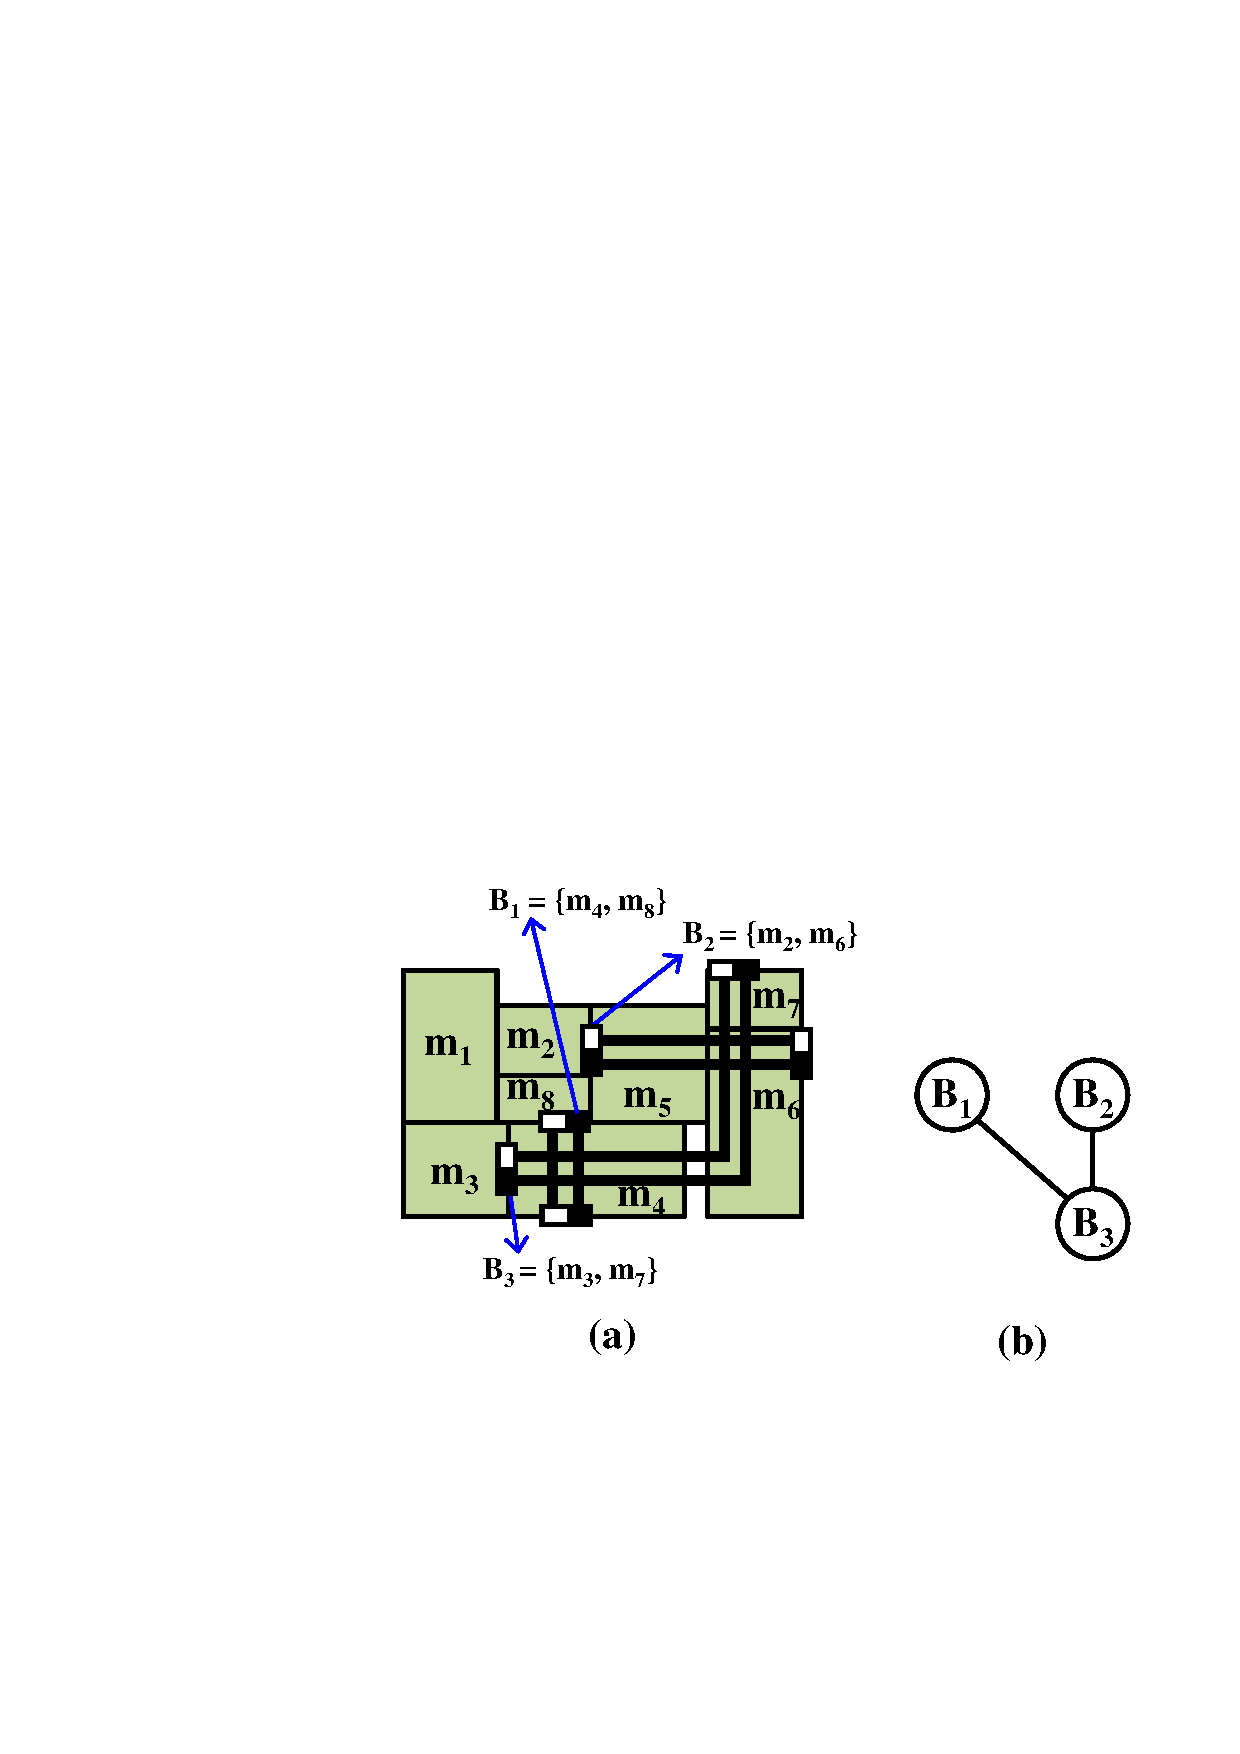
\includegraphics[width=11cm]{Fig/layer_assignment.pdf}
    %\centerline{\psfig{figure=Fig/layer_assignment.eps, width=11cm}}
     \caption{
      Layer assignment.
   }
  \label{fig::layer_assignment}
\end{figure}

Figure~\ref{fig::layer_assignment} illustrates how the
algorithm works. In Figure~\ref{fig::layer_assignment}
(a), there are three buses and the modules passed by those
buses are shown in the brace. The conflict graph is given in
Figure~\ref{fig::layer_assignment} (b).
Due to the bend of diagonal bus $B_3$ occurs at the module which is
not a bus module, it must assign the bus components of the bus $B_3$
to the same layer. Thus, the diagonal bus $B_3$ is represented as the node $B_3$ in the graph.
Initially, the node $B_3$ has the maximum degree in the conflict graph.
We assign it to layer one, and all its neighbors $B_1$ and $B_2$ are assigned
to layer two. Then it terminates because all buses are assigned to one of the two layers.
Figure~\ref{fig::layer_assignment}(c) is the result of layer
assignment, the nodes in layer one are marked with white color,
and the nodes in layer two are marked with black color.

\section{Orientation Determination
and Deviation Minimization}
\label{sec::Orientation Determination}
\subsection{Deviation Minimization with Lookup Table Method}
\label{sec::Deviation Minimization with Lookup Table Method}
%deviation optimization
\begin{figure}[htb]
  \centering
    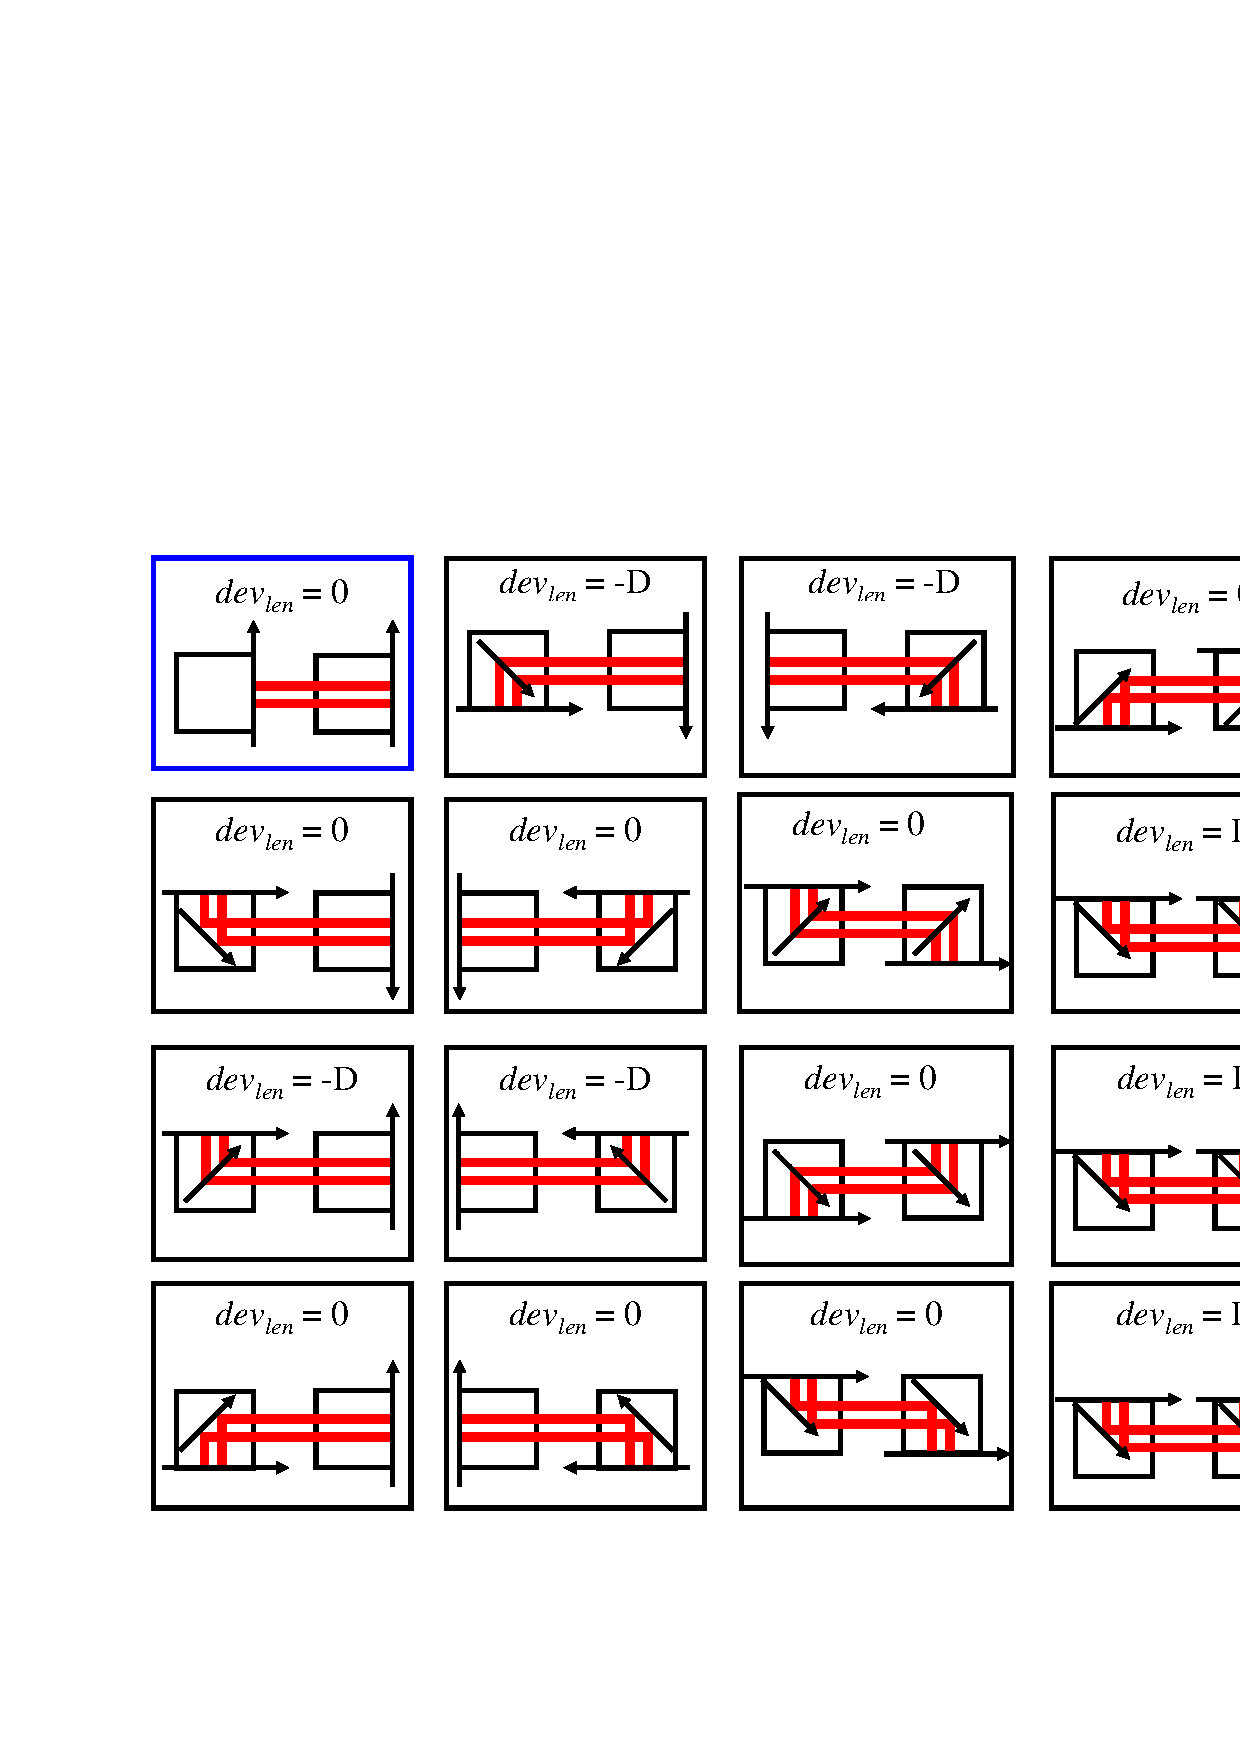
\includegraphics[width=12cm]{Fig/total_deviation_pattern.pdf}
    %\centerline{\psfig{figure=Fig/total_deviation_pattern.eps, width=12cm}
     \caption{
      Total possible bus shapes between any two modules.
   }
  \label{fig::total_deviation_pattern}
\end{figure}

The bus routing problem has attracted much attention recently, and
one of the popular problems is to determine the bus orientation
and minimize the deviation at each load \cite {Mo07_1, Mo07_2}.
However, these works mainly consider the impact of the blockages
during bus routing that have different objective with ours.
Besides, extra vias at the bend of each diagonal bus component
is allowed in the above works, however, the vias have adverse
effects on the bus delay, it is \textbf{\textit{forbidden}} under
our problem formulation.
Therefore, we develop a new algorithm that can be integrated into
our bus-driven floorplanner.

\begin{figure}[htb]
  \centering
    \includegraphics[width=9cm]{Fig/deviation_pattern1.pdf}
    %\centerline{\psfig{figure=Fig/deviation_pattern1.eps, width=10cm}}
  \centering
    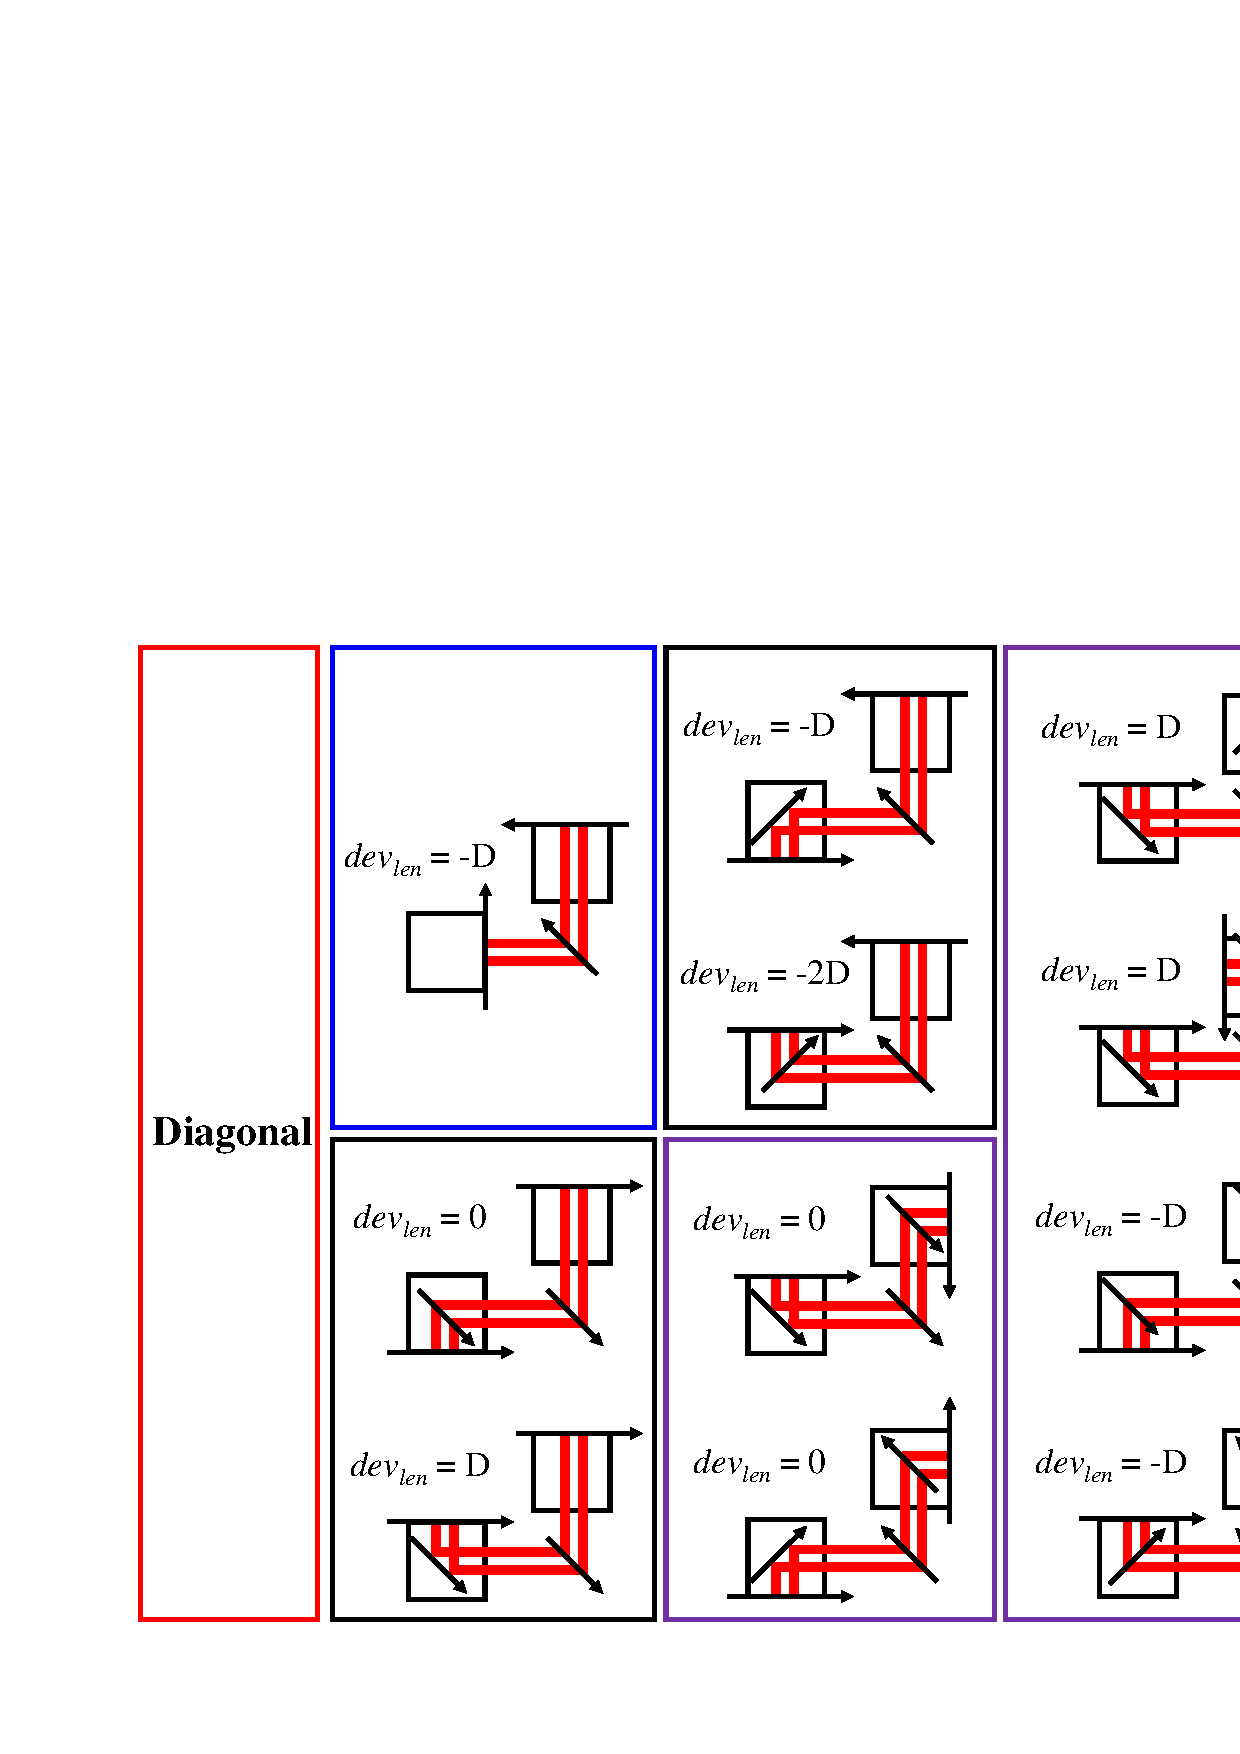
\includegraphics[width=12cm]{Fig/deviation_pattern2.pdf}
    %\centerline{\psfig{figure=Fig/deviation_pattern2.eps, width=13cm}}
     \caption{
      The bus patterns derived from the horizontal, vertical, and diagonal connections.
   }
  \label{fig::deviation_pattern1}
\end{figure}

In this paper, we explore all possible bus shapes including the position of the bus pin
between any two modules, and obtain total 150 possible bus shapes,
part of the total possible bus shapes are illustrated in Figure~\ref{fig::total_deviation_pattern}.
Different bus shapes can be mapped to some general patterns by mirroring or rotating,
finally, total 24 bus patterns are concluded. Given the initial position
of the bus pins on the modules, it can obtain the possible
patterns. Next, according to the accumulated deviation at previous
module, it chooses the pattern holding the best accumulated
deviation at the module. Finally, the accumulated deviation at the
modules, the orientation and position of the bus pins, and the position of the bus pins
can be determined. Figure~\ref{fig::deviation_pattern1} shows the
24 concluded patterns. The arrows represent the position and
orientation of the bus pins at the turning
nodes and the modules. Different cases can contribute different deviations.

\begin{figure}[htb]
  \centering
    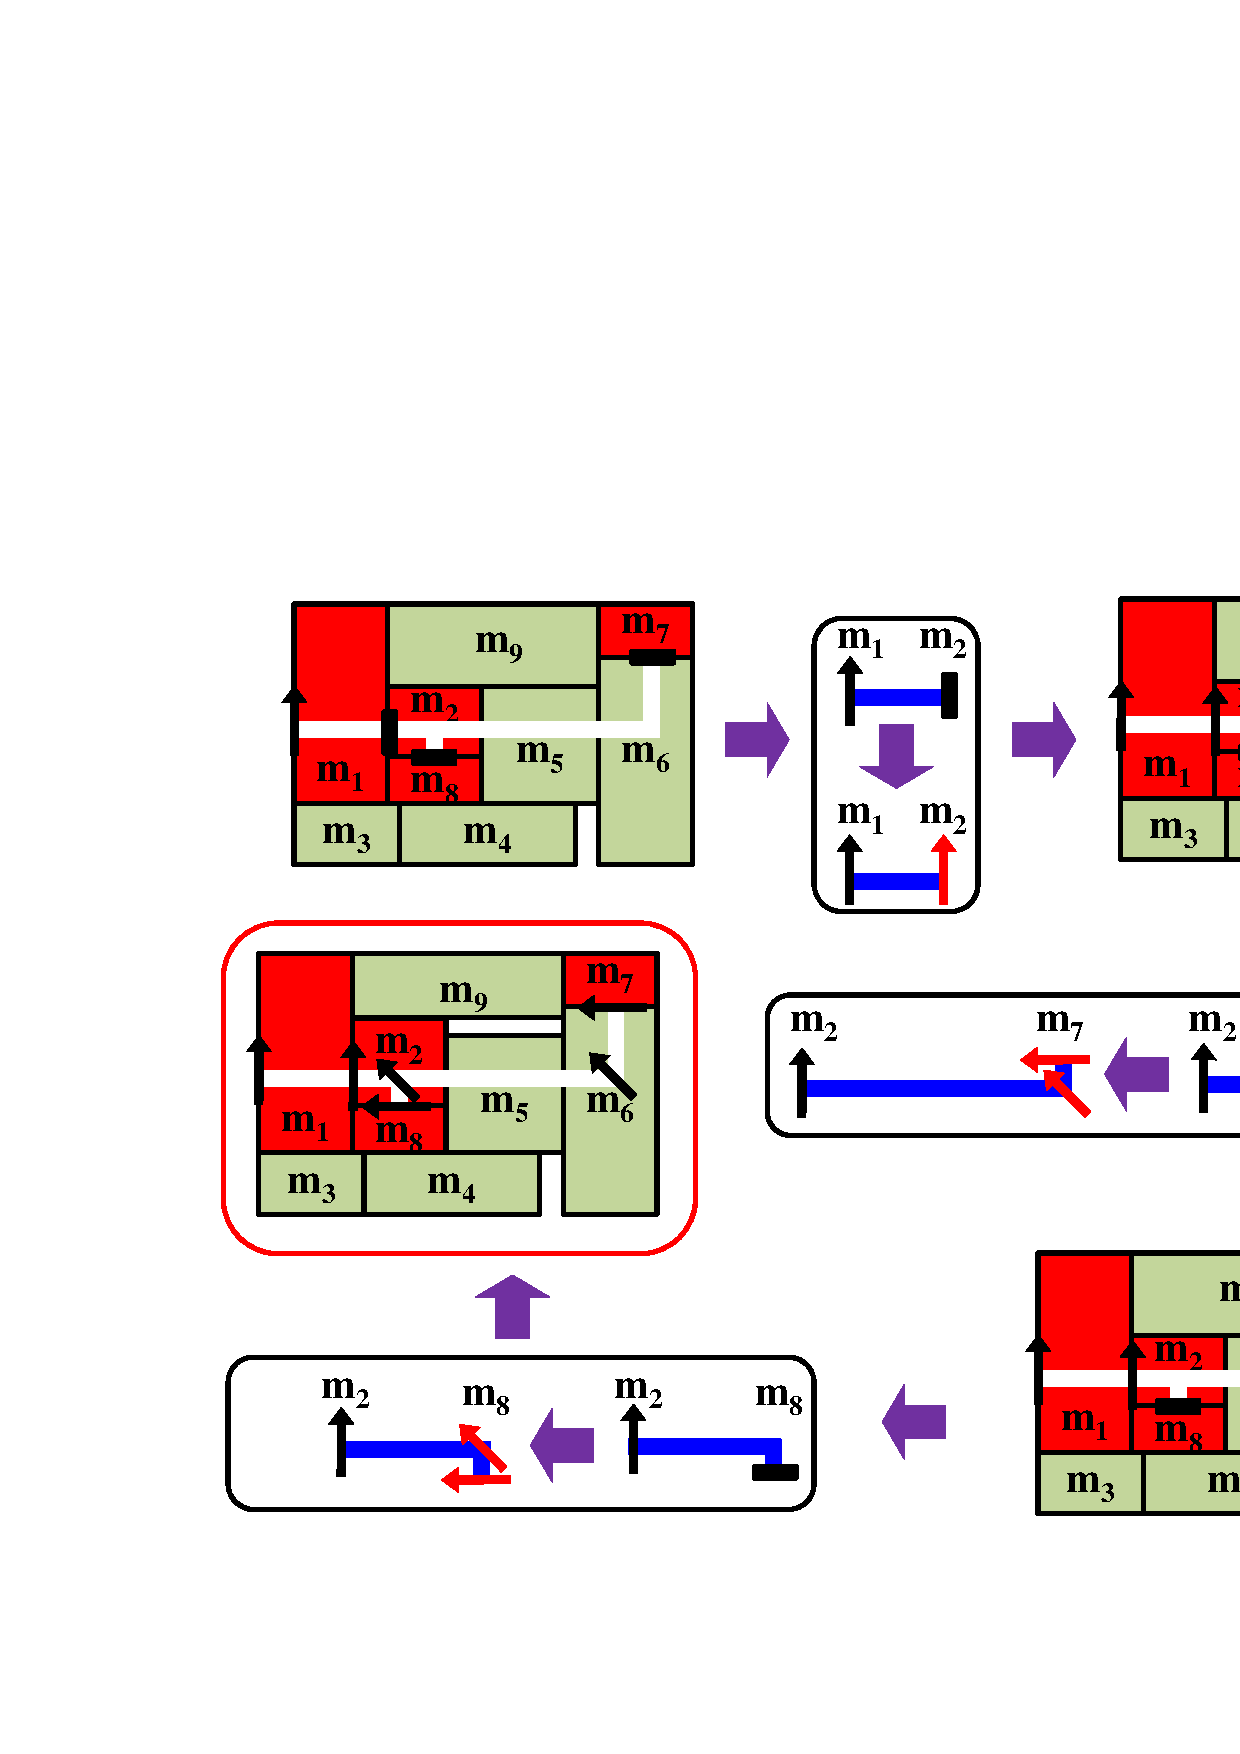
\includegraphics[width=12cm]{Fig/deviation_example1.pdf}
    %\centerline{\psfig{figure=Fig/deviation_example1.eps, width=12cm}}
     \caption{
      Determine the orientation and deviation for all bus pins and turning nodes.
   }
  \label{fig::deviation_example1}
\end{figure}

Figure~\ref{fig::deviation_example1} illustrates how the
algorithm works. There is a bus which passes through the modules in
\{$m_1$, $m_2$, $m_7$, $m_8$\}, each module holds the initial
position of the bus pins, and their orientation is not determined yet.
We assume that $m_1$ is the driver, the searching order obtained from
performing depth first search (DFS) on the MST is $m_1 \rightarrow m_2
\rightarrow m_7 \rightarrow m_8$. The deviation of the driver $m_1$ is 0.
First, the module $m_2$ is picked as the candidate.
The modules $m_1$ and $m_2$ are connected with
a horizontal bus component passing through the bus pins on the modules, so
it can obtain one possible pattern from the 24 concluded patterns.
The obtained pattern contributes 0 at the accumulated deviation, so the
accumulated deviation from the driver to module $m_2$ is still 0, then the
orientation of the bus pin on module $m_2$ is obtained.

Next, the module $m_7$ is chosen as the candidate. The modules $m_2$ and $m_7$
are connected with the diagonal bus component passing through the bus pins on
the modules, so it can obtain one possible pattern from the
24 concluded patterns. The obtained pattern contributes $-$D at the
accumulated deviation, so the accumulated deviation from the
driver to the module $m_7$ is $-$D, then the orientations of the bus
pin on the module $m_7$ and the turning node are obtained.

Finally, the module $m_8$ is selected as the candidate. The modules $m_2$
and $m_8$ are connected with only one vertical bus component. However, the
bus pin on the module $m_2$ is not passed by the
vertical bus component, so it can obtain two possible patterns from the
24 concluded patterns. One pattern contributes 0 at the
accumulated deviation of the module, and another pattern contributed $-$D at the
accumulated deviation of the module. Since the accumulated deviation from the
driver to the previous module $m_2$ is 0, the pattern contributing
0 at the accumulated deviation of the module is chosen. Then the accumulated
deviation from the driver to the module $m_8$ is 0, the orientations of
the bus pin on the module $m_8$ and the turning
node are obtained.
Now the algorithm terminates because the
position and orientation of all bus pins are determined.

\subsection{Fast Deviation Update Based on Topology Comparison}
\label{sec::Fast Deviation Update Based on Topology Comparison}

To decrease the time for searching possible patterns, we propose another approach
which divides the procedure of determining the deviation of each
module into two steps --- deviation determination and accumulated deviation (AD) update.
In each iteration, the AD can be quickly updated after the deviation of the candidate is determined.
Since the process of determining the deviation of each
module is split, the shorter segment is needed for each comparison during searching the best pattern.
If the bus pin on different modules can be connected by one straight line, then its deviation is equal to its AD,
therefore, and those bus patterns are unnecessary kept in the concluded bus patterns.
Finally, total 24 bus patterns can be further reduced to 10 types.
\begin{figure}[htb]
  \centering
    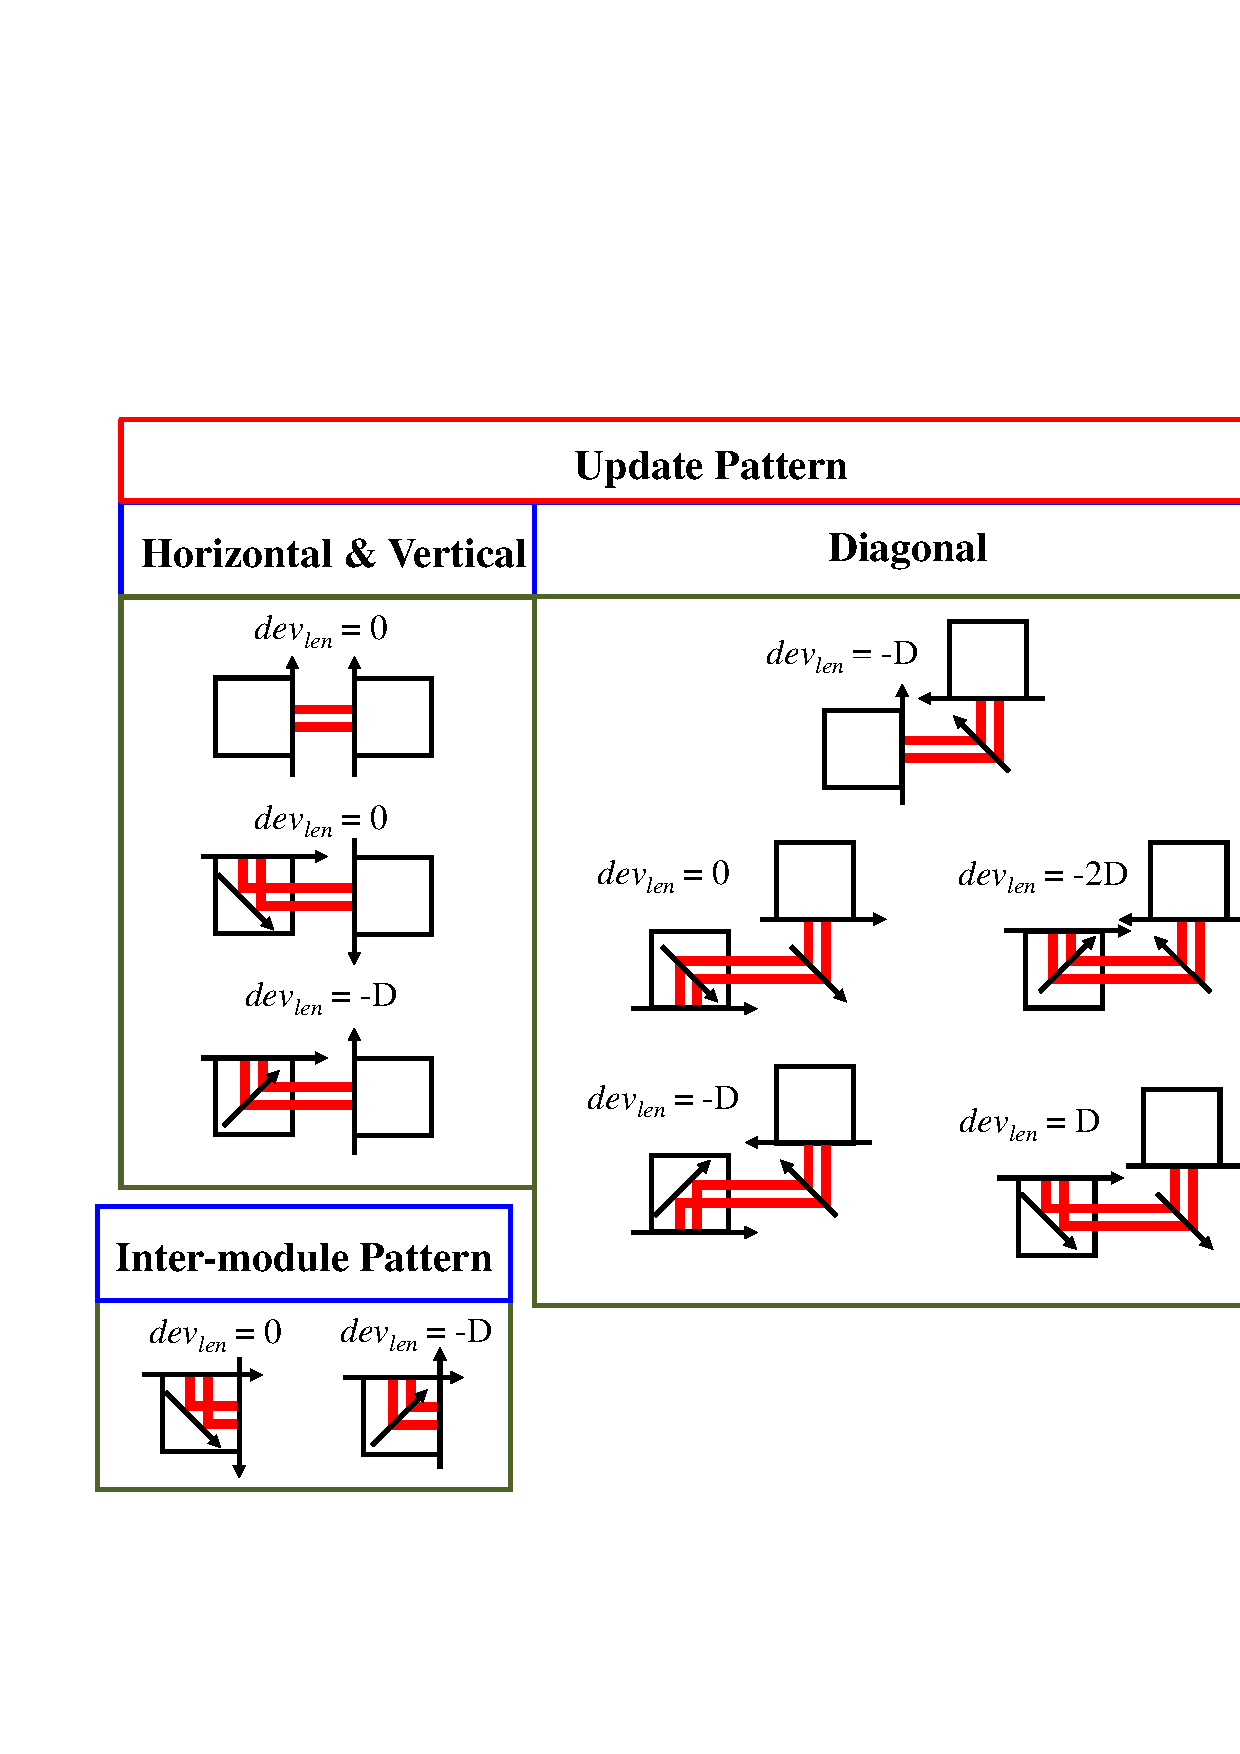
\includegraphics[width=11cm]{Fig/deviation_reduced_pattern.pdf}
    %\centerline{\psfig{figure=Fig/deviation_reduced_pattern.eps, width=11cm}}
     \caption{
      The reduced bus patterns.
   }
  \label{fig::deviation_reduced_pattern}
\end{figure}

Figure~\ref{fig::deviation_reduced_pattern} gives total 10 concluded
bus patterns. The deviation of each candidate is determined from the inter-module patterns, and the update patterns
are used to update the AD of its neighbors.
In this algorithm, the candidate is chosen based on the searching order which is obtained by performing
breadth first search (BDF) on the MST, if a module has at least two neighbors, the neighbors are selected clockwise from its upper side.

\begin{figure}[htb]
  \centering
    \includegraphics[width=11cm]{Fig/deviation_calculation.pdf}
    %\centerline{\psfig{figure=Fig/deviation_calculation.eps, width=11cm}}
     \caption{
      The procedure of deviation determination and AD update.
   }
  \label{fig::deviation_calculation}
\end{figure}

Figure~\ref{fig::deviation_calculation} shows how the algorithm works.
Initially, the bus pin of the candidate is placed on its upper boundary.
Based on different AD on the module, the best deviation and orientation can be obtained from the inter-module patterns.
We assume that the best deviation can be obtained at the candidate if the bus pin is placed on its upper boundary,
then segment 1 and segment 2 are chosen to determine the deviation at the candidate.
According to different relative positions between the candidate and its neighbors,
it finds the matched pattern with segment 1, segment 3, and segment4 from the update patterns,
then the AD of its neighbors can be obtained.

\begin{figure}[htb]
  \centering
    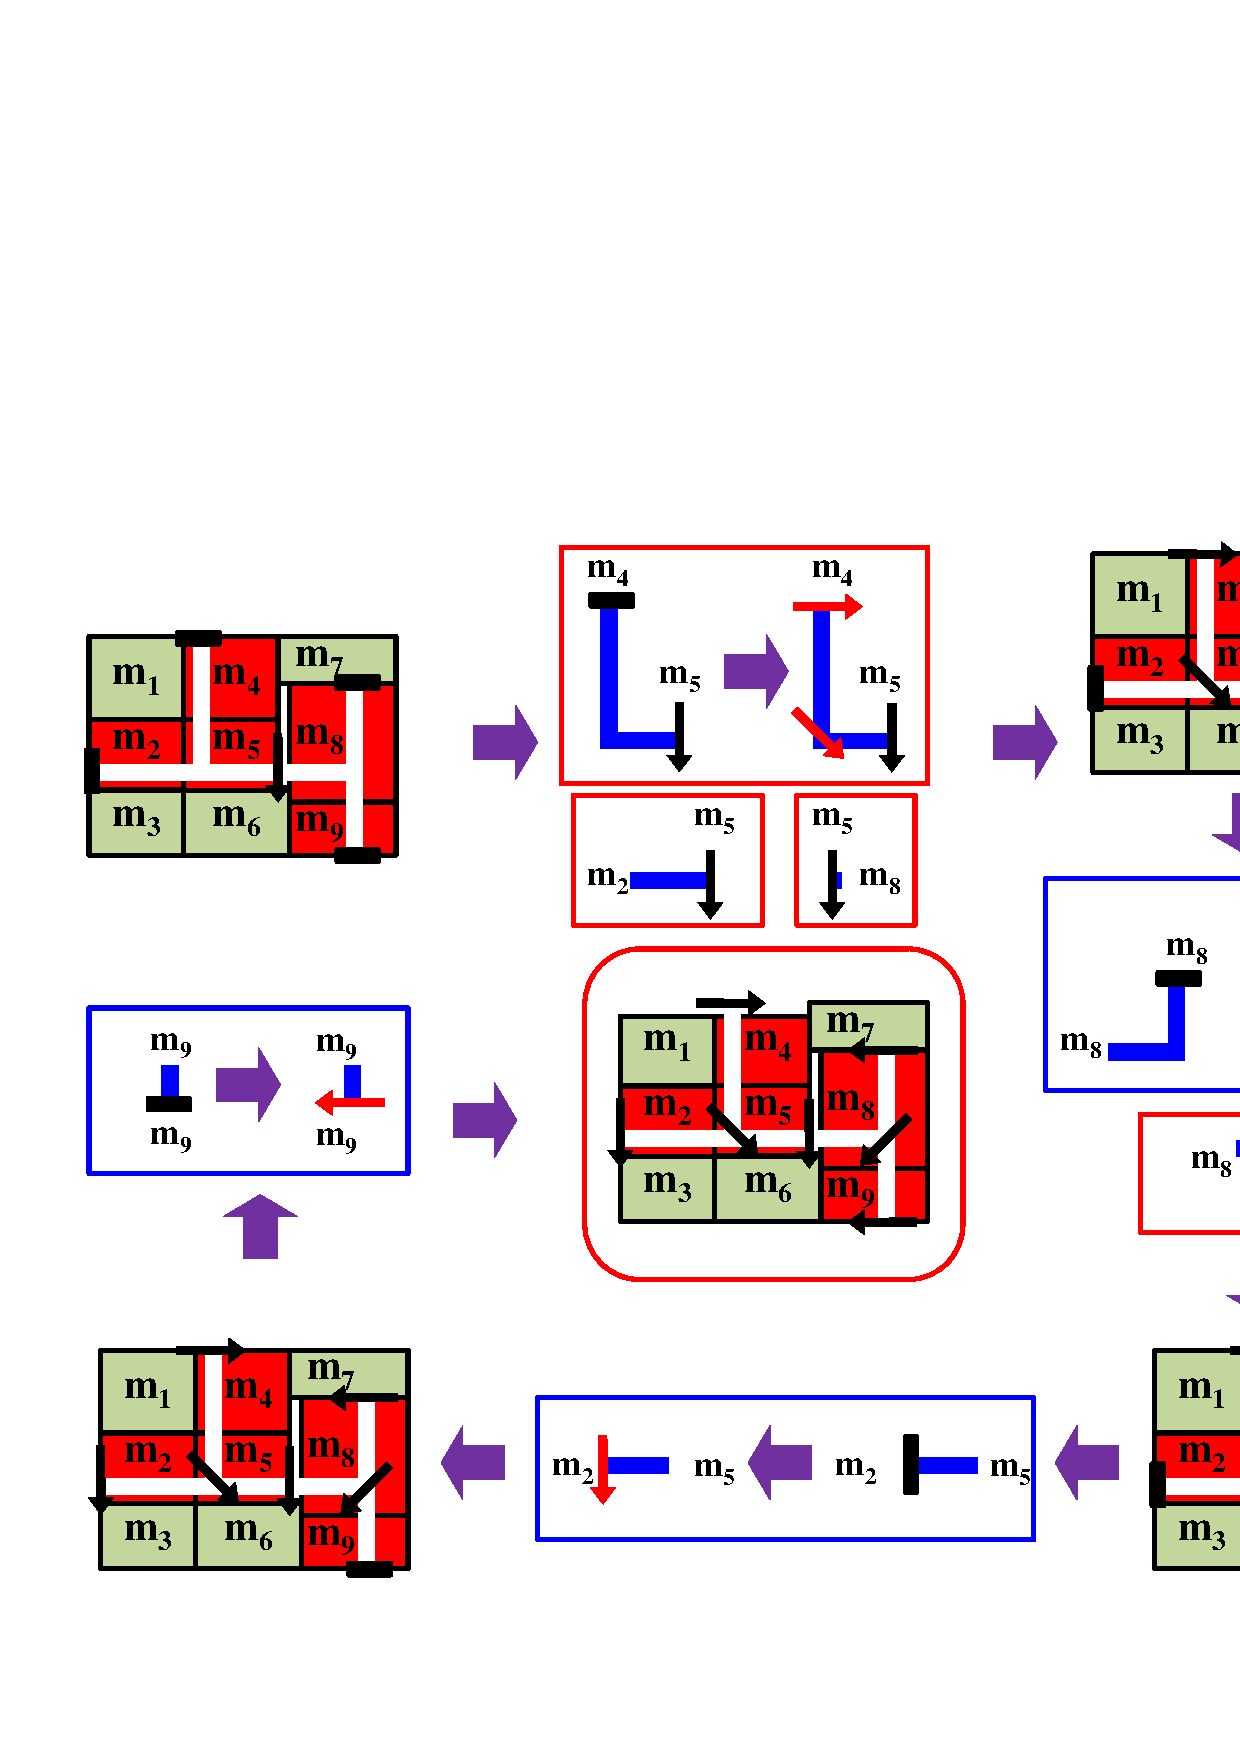
\includegraphics[width=13cm]{Fig/deviation_example2.pdf}
    %\centerline{\psfig{figure=Fig/deviation_example2.eps, width=13cm}}
     \caption{
      Determine the orientation and deviation for all bus pins and turning nodes.
   }
  \label{fig::deviation_example2}
\end{figure}

Figure~\ref{fig::deviation_example2} gives an example to illustrate how the algorithm works.
There is a bus which passes through the modules in
\{$m_2$, $m_4$, $m_5$, $m_8$, $m_9$\}, each module holds the initial
position of the bus pins, and their orientation is not determined yet. We assume that $m_5$ is
the driver, the searching order obtained from performing BFS on the MST is $m_5 \rightarrow m_4
\rightarrow m_8 \rightarrow m_2 \rightarrow m_9$. First, the module $m_5$ is
picked as the candidate. Since $m_5$ is the driver, its deviation is 0, then the AD of its neighbors
are updated based on their relative positions.
First, the best pattern from the update patterns is chosen to determine the orientation at the turning nodes in the driver,
then the orientation and position of the bus pin on module $m_4$, the deviation at the module $m_4$ could be obtained.
Next, it updates the AD for the modules $m_8$ and $m_2$. In next iteration, the module $m_4$ is selected as the candidate.
However, the deviation at the module $m_4$ is obtained and it has no neighbor,
the next module in the searching order is chosen to continue the procedure.
In next iteration, the module $m_8$ is selected as the candidate.
It first finds the best pattern from the inter-module patterns to determine its deviation.
Then it updates AD for its neighbors $m_9$. In next iteration, the module $m_2$ is chosen as the candidate.
Since the bus pin on module $m_2$ is connected by only one straight bus line, its deviation is equal to
its AD. Finally, it selects the module $m_9$ as the candidate, the deviation of the module $m_9$ is equal to
its AD because the bus pin is connected by only one straight bus line.
Now the algorithm terminates because the position and orientation of all bus pins are determined.

\begin{figure}[htb]
  \centering
    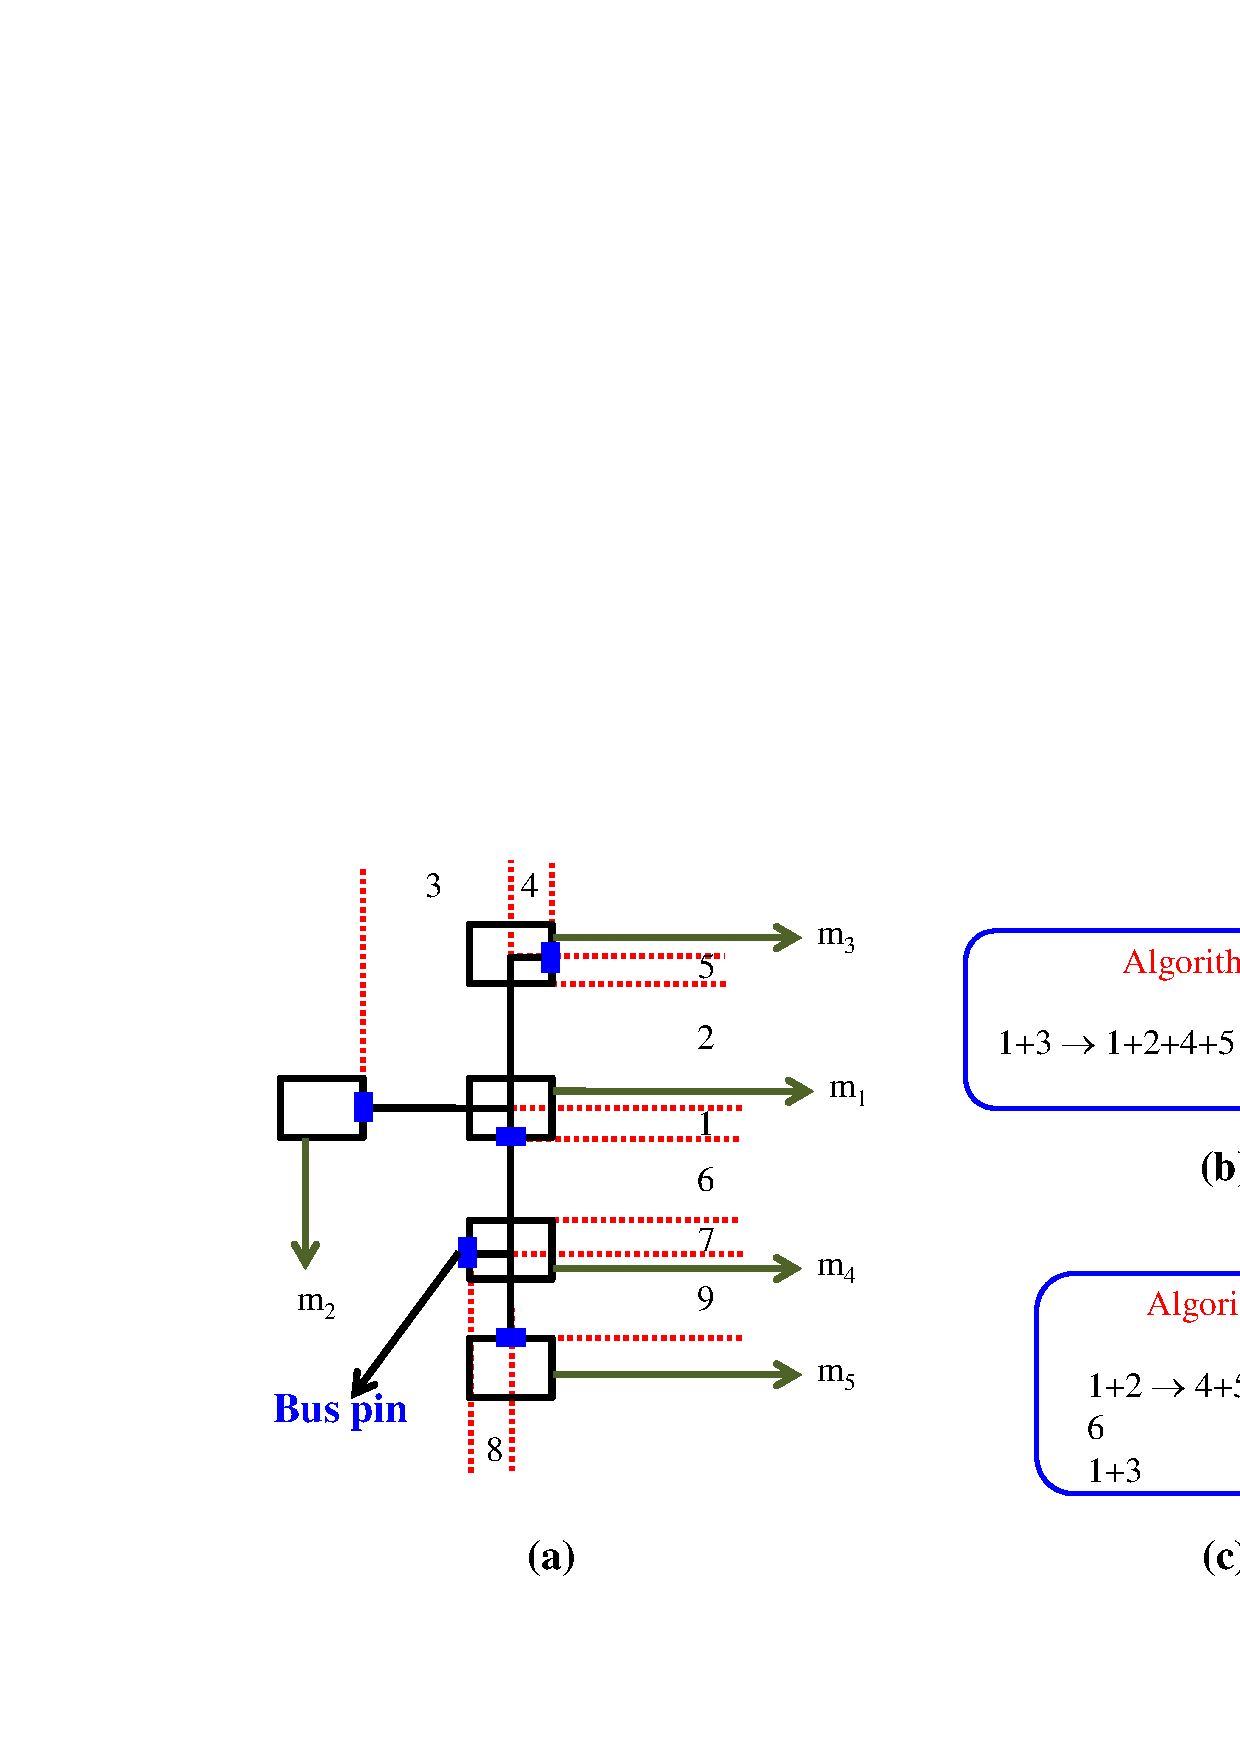
\includegraphics[width=13cm]{Fig/algorithm_comparison.pdf}
    %\centerline{\psfig{figure=Fig/algorithm_comparison.eps, width=13cm}}
     \caption{
      The difference between two algorithms.
   }
  \label{fig::algorithm_comparison}
\end{figure}

We use Figure~\ref{fig::algorithm_comparison} to demonstrate the difference between two algorithms.
In Figure~\ref{fig::algorithm_comparison} (a), there are five modules connected with one bus and each bus segment is marked as a number.
The module $m_1$ is the driver. For the first algorithm, we assume the searching order is $m_1 \rightarrow m_2 \rightarrow m_3 \rightarrow m_4 \rightarrow m_5$,
the sequence of the bus segments which is processed during the algorithm is shown in Figure~\ref{fig::algorithm_comparison} (b).
As for the second algorithm, the searching order is $m_1 \rightarrow m_3 \rightarrow m_4 \rightarrow m_2 \rightarrow m_5$,
the sequence of the bus segments which is processed during the algorithm is shown in Figure~\ref{fig::algorithm_comparison} (c).

As given in Figure~\ref{fig::algorithm_comparison} (b) and Figure~\ref{fig::algorithm_comparison} (c),
it shows that the bus patterns are more complicated in first algorithm than in second algorithm, thus,
the number of the possible bus patterns in first algorithm are more than the number of the possible bus patterns in second algorithm,
and it will spend more time to search for a best pattern.

\begin{Lemma}
For some specific bus topologies in the candidate, the AD of its neighbors can be
directly calculated without searching for the best bus pattern.
\end{Lemma}

\begin{figure}[htb]
  \centering
    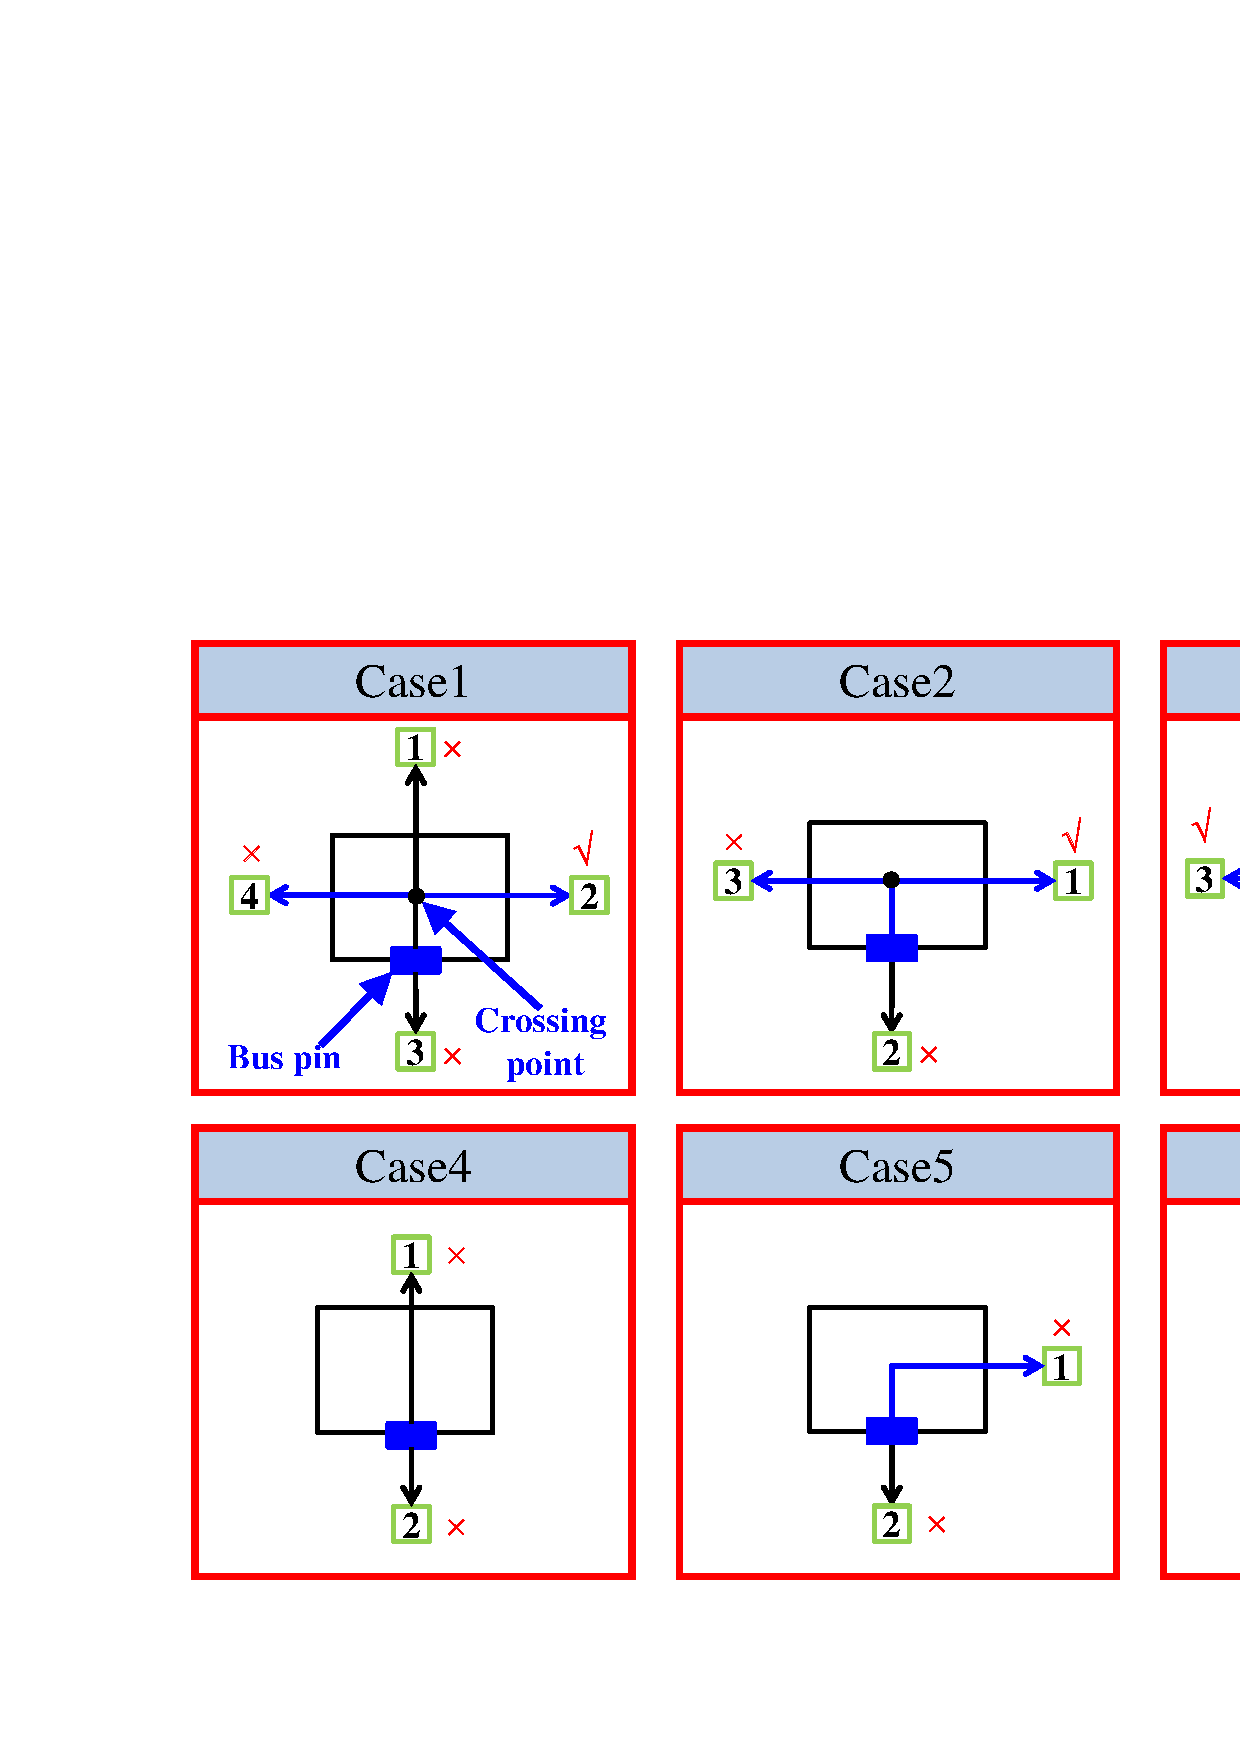
\includegraphics[width=11cm]{Fig/deviation_driver.pdf}
    %\centerline{\psfig{figure=Fig/deviation_driver.eps, width=11cm}}
     \caption{
      All possible topologies in driver.
   }
  \label{fig::deviation_driver}
\end{figure}

In the following, several cases will be analyzed under different conditions.
As shown in Figure~\ref{fig::deviation_driver}, there are total six possible topologies
in the driver, all other topologies can be mapped to these six cases by rotating or mirroring.
In case 1, the driver has four neighbors.
Since the modules at the direction 1 and direction 3 are connected by one straight line to
the bus pin of the driver. There is no deviation contributed by the driver.
The AD of the module at the direction 1 and direction 3 are determined by the relation position between the driver and it.
If the modules at the direction 1 and direction 3 are connected by one diagonal bus with the driver, then it will contribute D or -D to the AD of the module.
The deviation of the modules at the direction 2 will be determined by finding the best
pattern from the update patterns as shown in Figure~\ref{fig::deviation_reduced_pattern},
then the best orientation at the crossing point can be obtained.
Since the orientation at the crossing point have been obtained, the AD of the module at the direction 4
can be calculated based on the orientation at the crossing point
and the relative position between the driver and it.
The directions are attached a tick mark if it needs to search the best bus pattern,
and the directions are attached a cross mark if the AD of the module can be directly calculated.
All other cases can be derived similarly.

Through the above cases, it can get the following conclusion:
since the neighbors of the candidate are processed in the clockwise from the north side,
if the bus pin on the driver is oriented horizontally and the driver has a right neighbor,
then the deviation at the right neighbor is obtained by searching the best pattern from the update patterns,
or the bus pin on the driver is oriented horizontally and the driver has only a left neighbor,
then the deviation at the left neighbor is obtained by searching the best pattern from the update patterns.
However, if the bus pin on the driver is oriented vertically and the driver has a upper neighbor,
then the deviation at the upper neighbor is obtained by searching the best pattern from the update patterns,
or the bus pin on the driver is oriented vertically and the driver has only a lower neighbor,
then the deviation at the lower neighbor is obtained by searching the best pattern from the update patterns.
After obtaining the orientation of the crossing point, the modules at other directions can be directly calculated
based on the obtained orientation and the relative position between the driver and it.

\begin{figure}[htb]
  \centering
    \includegraphics[width=11cm]{Fig/deviation_load.pdf}
    %\centerline{\psfig{figure=Fig/deviation_load.eps, width=11cm}}
     \caption{
      All possible topologies in load.
   }
  \label{fig::deviation_load}
\end{figure}

In Figure~\ref{fig::deviation_load}, there are total six possible topologies
in the load. The $``$\textbf{\textit{S}}$"$ stands for the accumulated direction of the deviation
from the driver.
The rule can be derived in the same way when the candidate is the driver.
If one neighbor of the candidate is at the first orthogonal direction compared with the accumulated direction
and the orientation of the crossing point is still not determined,
then the deviation of the neighbor is obtained by searching the best pattern from the update patterns,
after that, the modules at other directions will be directly calculated based on the obtained orientation and the
relative position between the driver and it.
According to the above rules, it will avoid unnecessary comparison, then the time for searching the best deviation will be minimized.

\section{Soft Module Adjustment} \label{sec::SOFT MODULE ADJUSTMENT}
In order to minimize the chip area, it adjusts the
dimension of some modules such that a better chip area can be
obtained. The adjustment is the same as that in \cite{Xiang03}.
The step is processed with another simulated annealing
process with the same cost function. In
each iteration of the annealing process, it chooses the module
lying on the critical path to change either its width or height a
little bit. However, if any feasible bus become invalid after
the adjustment, the candidate solution will be discarded.


\include{5/experiment}
% ------------------------------------------------
\StartChapter{Conclusion}{chapter:conclusion}
% ------------------------------------------------

% ------------------------------------------------
\EndChapter
% ------------------------------------------------


% ------------------------------------------------

% 附錄 Appendix

% ----------------------------------------------------------------------------
%                                 Appendix
%                                   附錄
% ----------------------------------------------------------------------------

% Page start
\newpage
\phantomsection

% ------------------------------------------------

% Appendix begins here
\appendix

% If more than one appendix chapters
%\appendices

% ------------------------------------------------

% ------------------------------------------------
% Page start
\newpage
\phantomsection
% ------------------------------------------------

\section{Li's Hash Project}

All source code and related data are open-source on \cite{web:lishash:home-page}.\\

This project will continuous to maintenance for any future work that basic on this design, so they can rely on it to do more and more research and development.\\

% ------------------------------------------------
% End of page
% ------------------------------------------------

\input{./appendix/appendix-2}

% ------------------------------------------------
% End of page
% ------------------------------------------------


% ------------------------------------------------

% 參考文獻 References

% ----------------------------------------------------------------------------
%                                 References
%                                   參考文獻
% ----------------------------------------------------------------------------

% Page start
\newpage
\phantomsection

% Add to "Table of Contents"
\addcontentsline{toc}{chapter}{References}

% Change the title of bibliography
\renewcommand\bibname{\centerline{References}}

% ------------------------------------------------

\bibliographystyle{abbrv}
\bibliography{./references/paper,./references/msic}

% ------------------------------------------------

% End of page

% ------------------------------------------------


% ------------------------------------------------

% End of paper
\end{document}

% ------------------------------------------------